\chapter{Implementacija i korisničko sučelje}
		
		
		\section{Korištene tehnologije i alati}
		
			%\textbf{\textit{dio 2. revizije}}
			
			% \textit{Detaljno navesti sve tehnologije i alate koji su primijenjeni pri izradi dokumentacije i aplikacije. Ukratko ih opisati, te navesti njihovo značenje i mjesto primjene. Za svaki navedeni alat i tehnologiju je potrebno \textbf{navesti internet poveznicu} gdje se mogu preuzeti ili više saznati o njima}.
			Za izradu dokumentacije korišten je alat \textbf{Texmaker}\footnote{\url{https://www.xm1math.net/texmaker/}} koji je razvojna okolina za jezik \textbf{LaTex}\footnote{\url{https://www.latex-project.org/}}. \textit{LaTex} je programski jezik za pisanje strukturiranih tekstova. Najčešće se koristi u oblikovanju znanstvenih radova.
			
			Dijagrami unutar dokumentacije izrađeni su pomoću alata \textbf{Astah UML}\footnote{\url{https://astah.net/}} i \textbf{lucid.app}\footnote{\url{https://lucid.app/}}. \textit{Astah UML} aplikacija je za modeliranje UML-a. \textit{Lucid.app} je web-stranica koja nudi isto to, no pristupačnija jer se ne mora preuzimati. Obje aplikacije se za studente ne naplaćuju.
			
			Komunikacija tima odvijala se preko aplikacije \textbf{WhatsApp}\footnote{\url{https://www.whatsapp.com/}}. Za potrebe ovog projekta bila je sasvim dovoljna, no za neke ozbiljnije projekte bilo bi potrebno prijeći na bolji alat.
			
			Kao sustav za upravljanje izvornim kodom korišten je \textbf{Git}\footnote{\url{https://git-scm.com/}}. Udaljeni repozitorij projekta je dostupan na web platformi \textbf{GitLab}\footnote{\url{https://gitlab.com/}}.
			
			Aplikacija je napisana u \textbf{Express}-u\footnote{\url{https://expressjs.com/}}, framework za izgradnju web-aplikacija na platformi \textbf{Node.js}\footnote{\url{https://nodejs.org/en/}}. Sve to je ostvareno programskim jezikom \textbf{Javascript}\footnote{\url{https://www.javascript.com/}}. \textit{Node.js} je back-end JavaScript runtime okruženje, radi na V8 JavaScript Engineu i izvršava JavaScript kod izvan web preglednika. 
			
			Sam kod aplikacije pisan je u proizvoljnom \textit{code editoru}, svi smo odabrali \textbf{Visual Studio Code}\footnote{\url{https://code.visualstudio.com/}}.
			
			Baza podataka je \textbf{PostgreSQL}\footnote{\url{https://www.postgresql.org/}} u oblaku na \textbf{Renderu}\footnote{\url{https://render.com/}}. Za lokalno korištenje baze korišten je alat \textbf{pgAdmin}\footnote{\url{https://www.pgadmin.org/}}. 
			
			\eject 
		
	
		\section{Ispitivanje programskog rješenja}
			
			%\textbf{\textit{dio 2. revizije}}\\
			
			% \textit{U ovom poglavlju je potrebno opisati provedbu ispitivanja implementiranih funkcionalnosti na razini komponenti i na razini cijelog sustava s prikazom odabranih ispitnih slučajeva. Studenti trebaju ispitati temeljnu funkcionalnost i rubne uvjete.}
	
			
			\subsection{Ispitivanje komponenti}
			%\textit{Potrebno je provesti ispitivanje jedinica (engl. unit testing) nad razredima koji implementiraju temeljne funkcionalnosti. Razraditi \textbf{minimalno 6 ispitnih slučajeva} u kojima će se ispitati redovni slučajevi, rubni uvjeti te izazivanje pogreške (engl. exception throwing). Poželjno je stvoriti i ispitni slučaj koji koristi funkcionalnosti koje nisu implementirane. Potrebno je priložiti izvorni kôd svih ispitnih slučajeva te prikaz rezultata izvođenja ispita u razvojnom okruženju (prolaz/pad ispita). }
			
			Ispitivanje komponenti proveli smo unutar Node.js tehnologije. U prva tri testa ispitivali smo funkcionalnosti trgovine. Testira se dohvaćanje imena trgovine preko ID-a, postojanje komentara za neku trgovinu i samo postojanje trgovine s nekim ID-jem.
			\begin{figure}[H]
			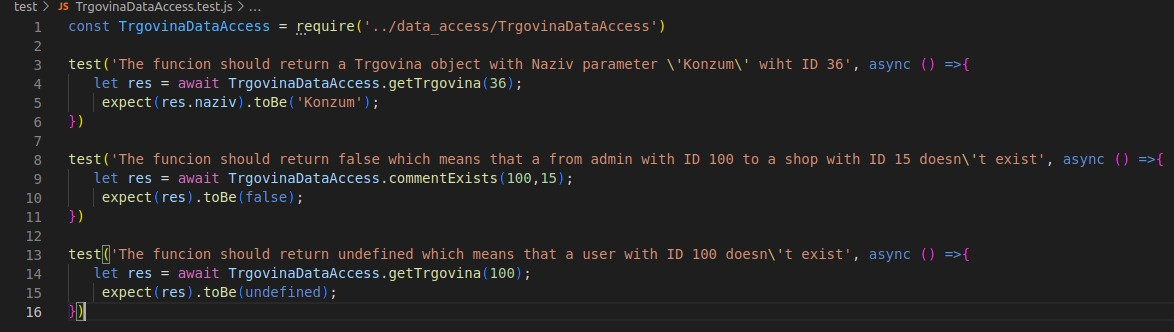
\includegraphics[width=\textwidth]{slike/test123.jpeg} %veličina u odnosu na širinu linije
			\caption{testovi 1, 2 i 3}
			\label{fig:test123} %label mora biti drugaciji za svaku sliku
			\end{figure}
			
			U druga tri testa ispitivale su se funkcionalnosti korisnika. Testiralo se postojanje korisnika s nekim ID-jem, dohvaćanje korisnika preko \textit{username}-a i nepostojanje korisnika s nevalidnim ID-jem.
			
			\begin{figure}[H]
			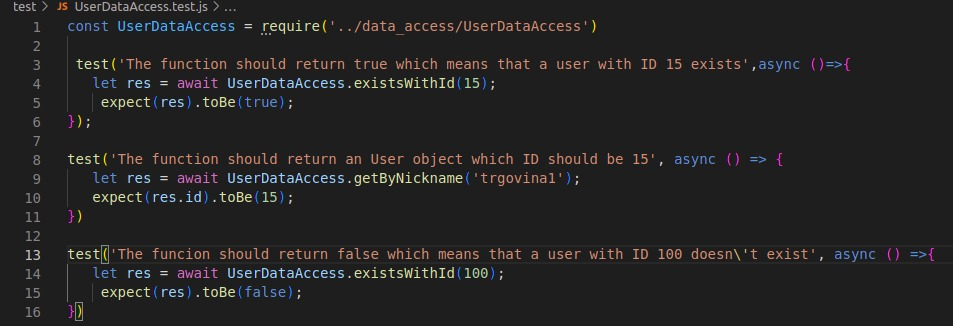
\includegraphics[width=\textwidth]{slike/test456.jpeg} %veličina u odnosu na širinu linije
			\caption{testovi 4, 5 i 6}
			\label{fig:test456} %label mora biti drugaciji za svaku sliku
			\end{figure}
			
			Svi testovi su prolazni i očekivano ponašanje aplikacije je postignuto.
			
			\begin{figure}[H]
			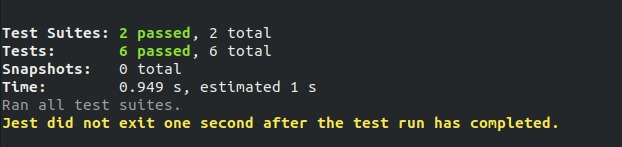
\includegraphics[width=\textwidth]{slike/reztest16.jpeg} %veličina u odnosu na širinu linije
			\caption{Rezultati testova}
			\label{fig:reztest16} %label mora biti drugaciji za svaku sliku
			\end{figure}
			
			
			
			
			
			
			\subsection{Ispitivanje sustava}
			
			 %\textit{Potrebno je provesti i opisati ispitivanje sustava koristeći radni okvir Selenium\footnote{\url{https://www.seleniumhq.org/}}. Razraditi \textbf{minimalno 4 ispitna slučaja} u kojima će se ispitati redovni slučajevi, rubni uvjeti te poziv funkcionalnosti koja nije implementirana/izaziva pogrešku kako bi se vidjelo na koji način sustav reagira kada nešto nije u potpunosti ostvareno. Ispitni slučaj se treba sastojati od ulaza (npr. korisničko ime i lozinka), očekivanog izlaza ili rezultata, koraka ispitivanja i dobivenog izlaza ili rezultata.\\ }
			 
			 %\textit{Izradu ispitnih slučajeva pomoću radnog okvira Selenium moguće je provesti pomoću jednog od sljedeća dva alata:}
			 %\begin{itemize}
			 %	\item \textit{dodatak za preglednik \textbf{Selenium IDE} - snimanje korisnikovih akcija radi automatskog ponavljanja ispita	}
			 	%\item \textit{\textbf{Selenium WebDriver} - podrška za pisanje ispita u jezicima Java, C\#, PHP koristeći posebno programsko sučelje.}
			% \end{itemize}
		 	%\textit{Detalji o korištenju alata Selenium bit će prikazani na posebnom predavanju tijekom semestra.}
		 	
		 	Prvi \textit{Selenium} test provodio se za funkcionalnosti \textbf{login}.
		 	
		 	\begin{figure}[H]
			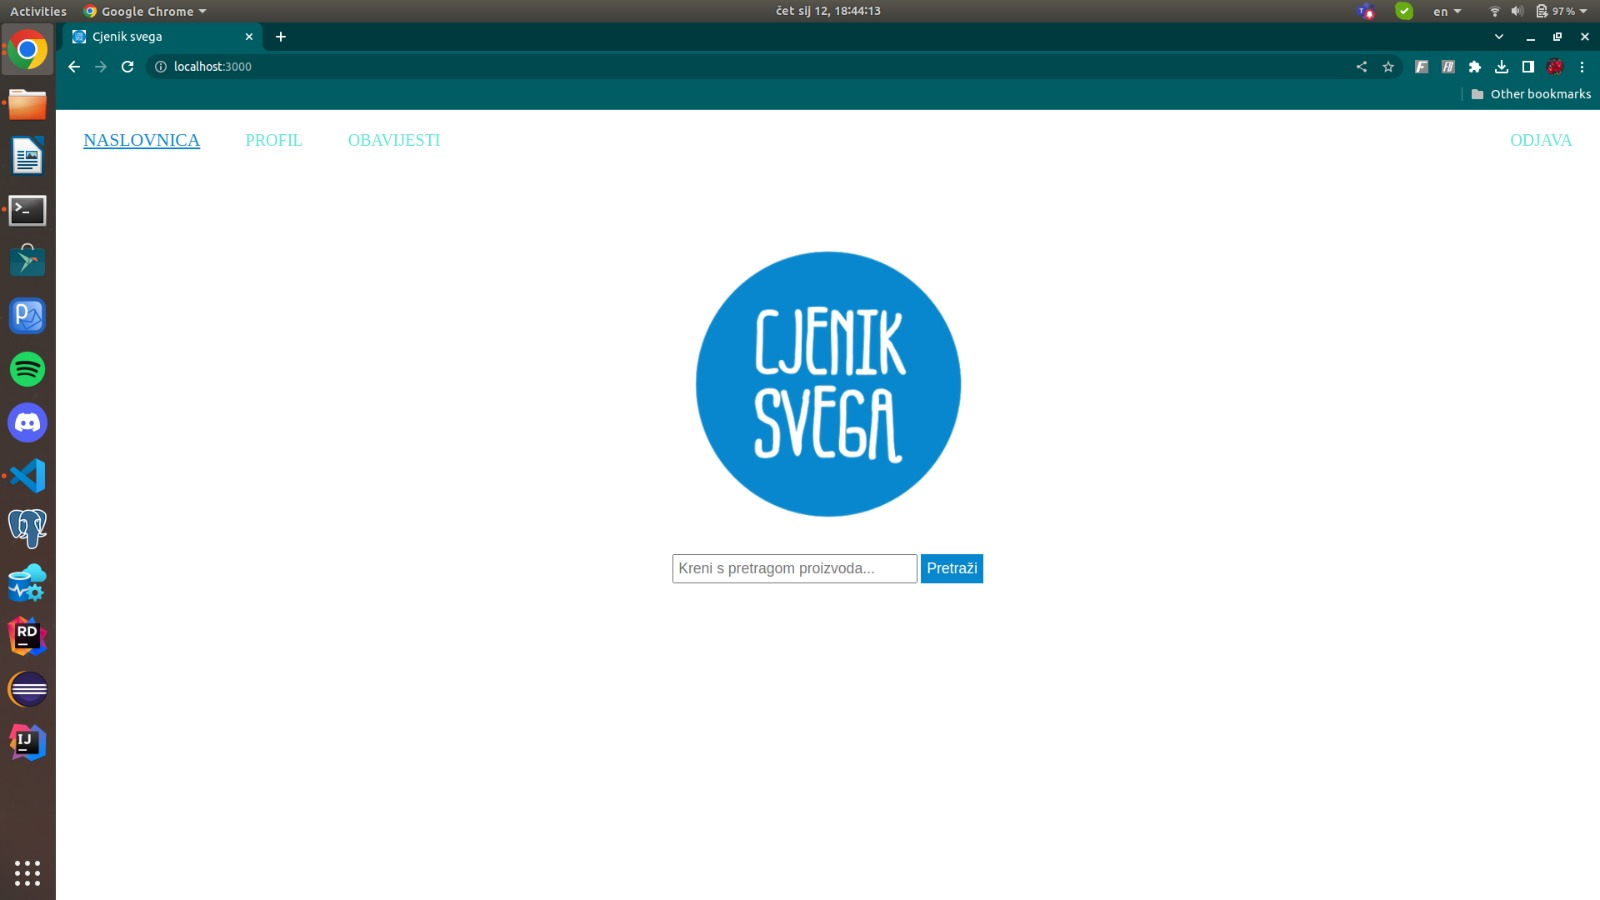
\includegraphics[width=\textwidth]{slike/sel1a.jpeg} %veličina u odnosu na širinu linije
			\caption{Selenium test 1, izgled sučelja}
			\label{fig:sel1a} %label mora biti drugaciji za svaku sliku
			Test je uspješan.
			\end{figure}
			\begin{figure}[H]
			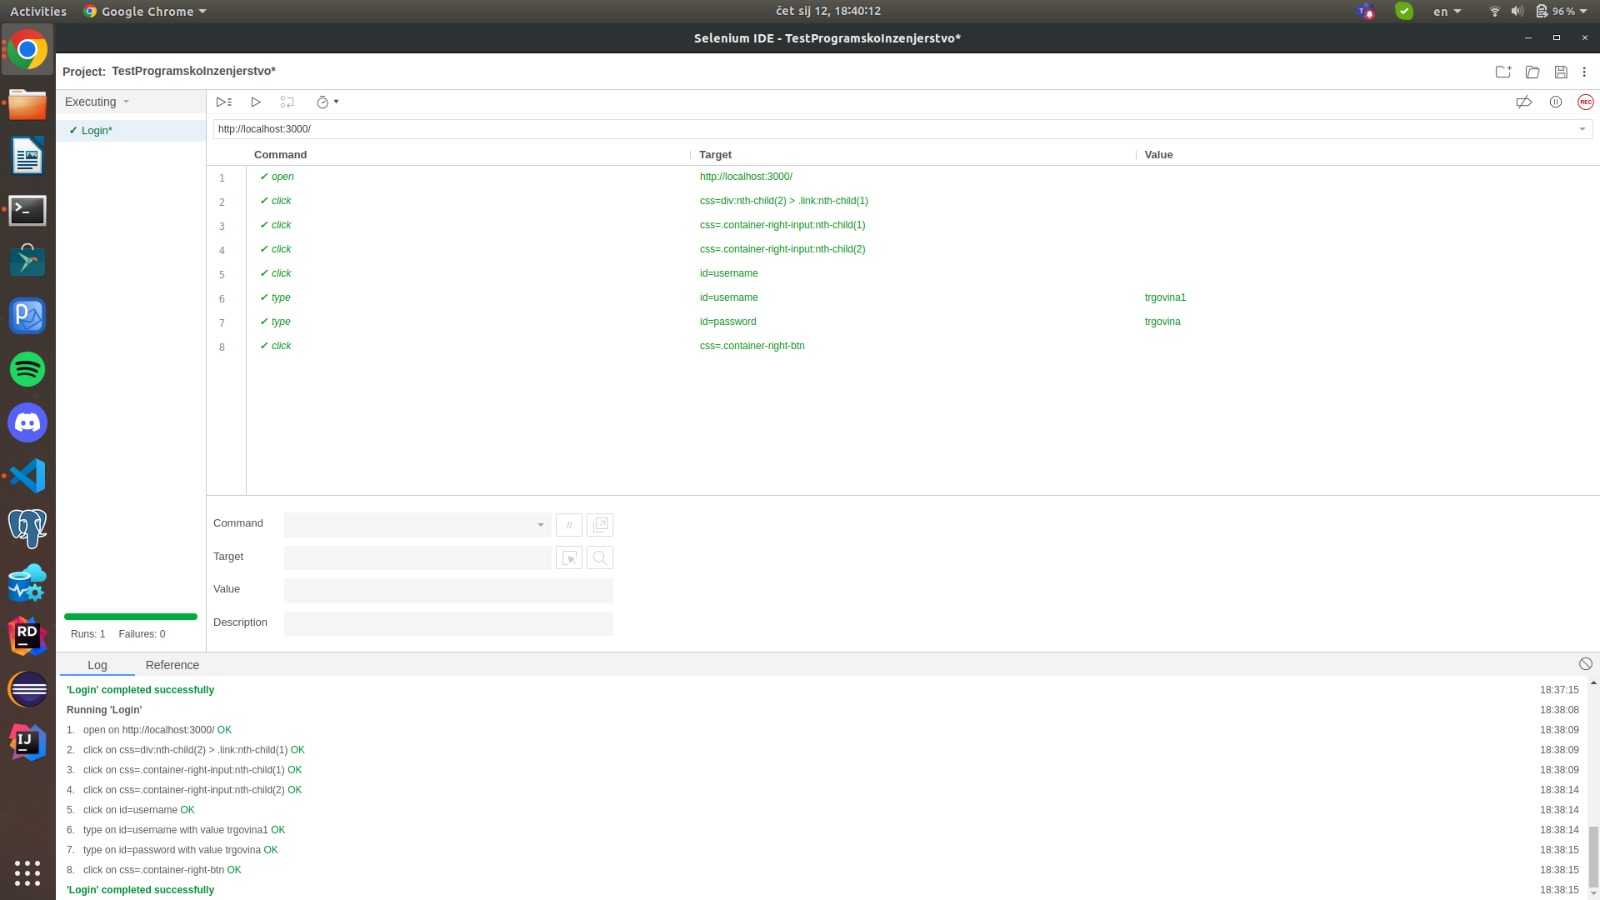
\includegraphics[width=\textwidth]{slike/sel1b.jpeg} %veličina u odnosu na širinu linije
			\caption{Selenium test 1, popis koraka}
			\label{fig:sel1b} %label mora biti drugaciji za svaku sliku
			\end{figure}
			
			Drugi \textit{Selenium} test provodio se za funkcionalnosti logina s krivom lozinkom. 
			
			\begin{figure}[H]
			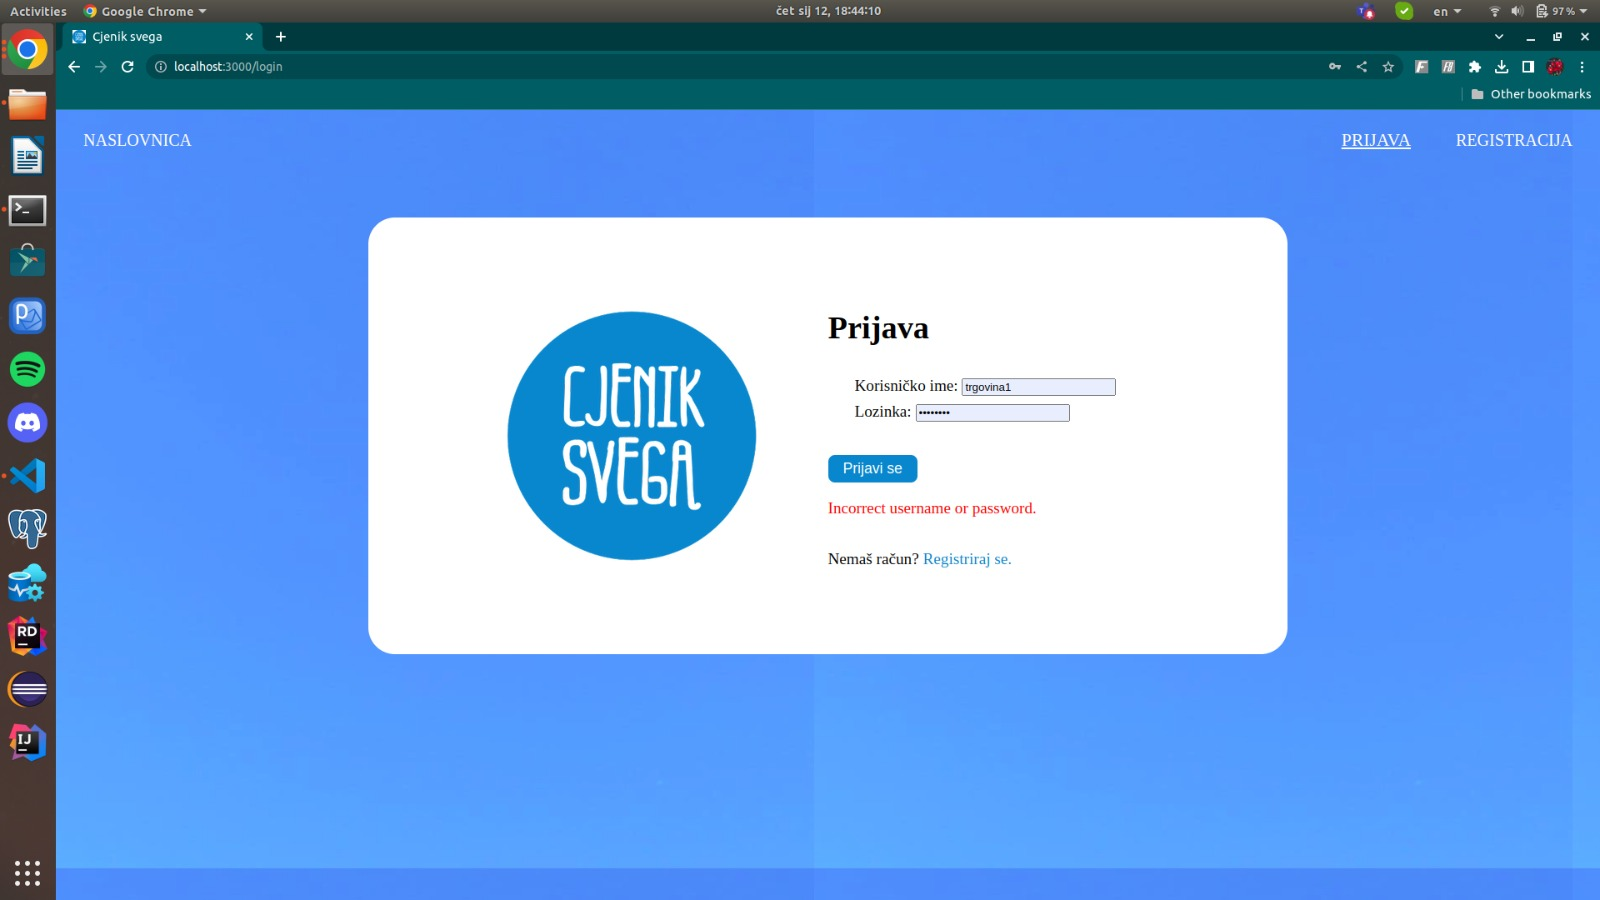
\includegraphics[width=\textwidth]{slike/sel2a.jpeg} %veličina u odnosu na širinu linije
			\caption{Selenium test 2, izgled sučelja}
			\label{fig:sel2a} %label mora biti drugaciji za svaku sliku
			Dobili smo očekivani rezultat.
			\end{figure}
			\begin{figure}[H]
			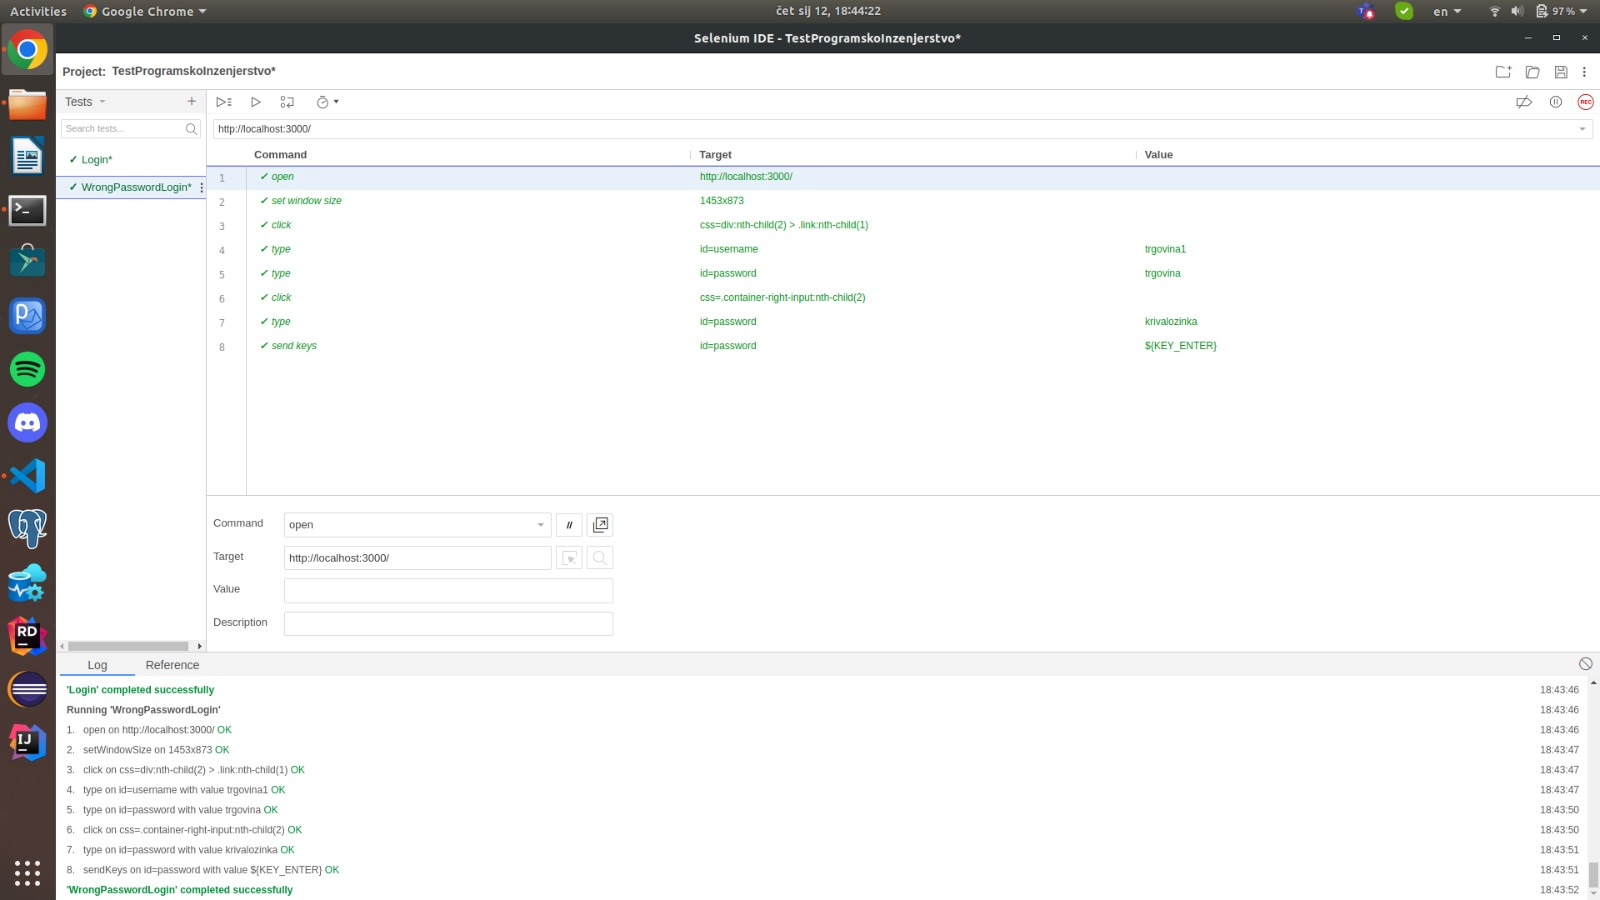
\includegraphics[width=\textwidth]{slike/sel2b.jpeg} %veličina u odnosu na širinu linije
			\caption{Selenium test 2, popis koraka}
			\label{fig:sel2b} %label mora biti drugaciji za svaku sliku
			\end{figure}
			
			Treći \textit{Selenium} test provodio se za funkcionalnosti pretraživanja proizvoda. Konkretno u testu pretraživali smo proizvod "banana". 
			
			\begin{figure}[H]
			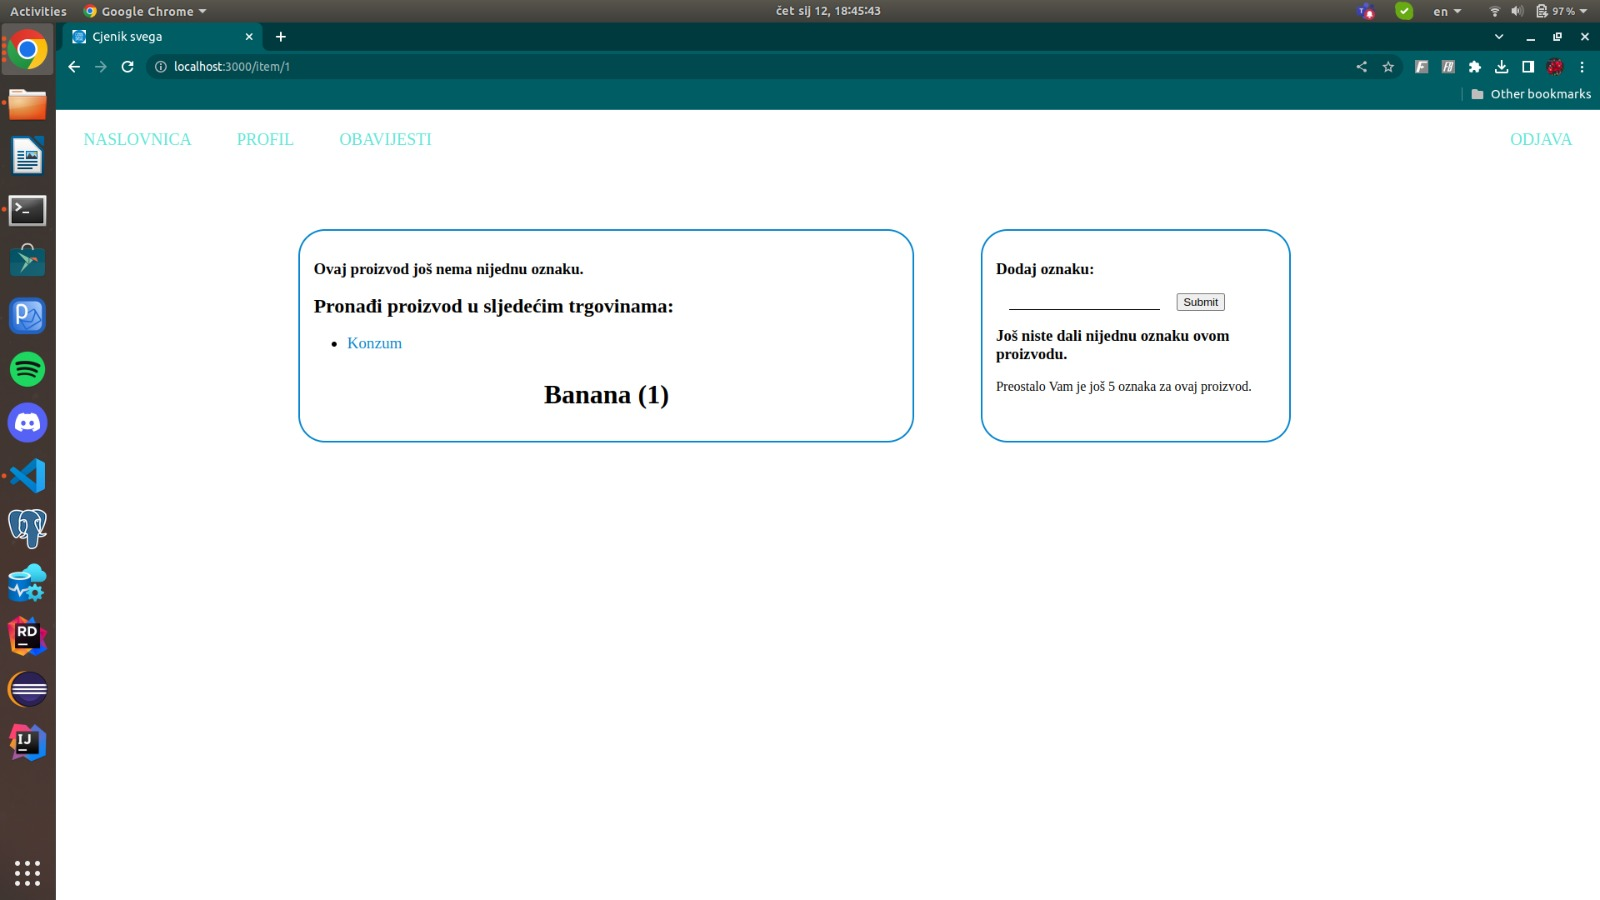
\includegraphics[width=\textwidth]{slike/sel3a.jpeg} %veličina u odnosu na širinu linije
			\caption{Selenium test 3, izgled sučelja}
			\label{fig:sel3a} %label mora biti drugaciji za svaku sliku
			Test je uspješan.
			
			\end{figure}
			\begin{figure}[H]
			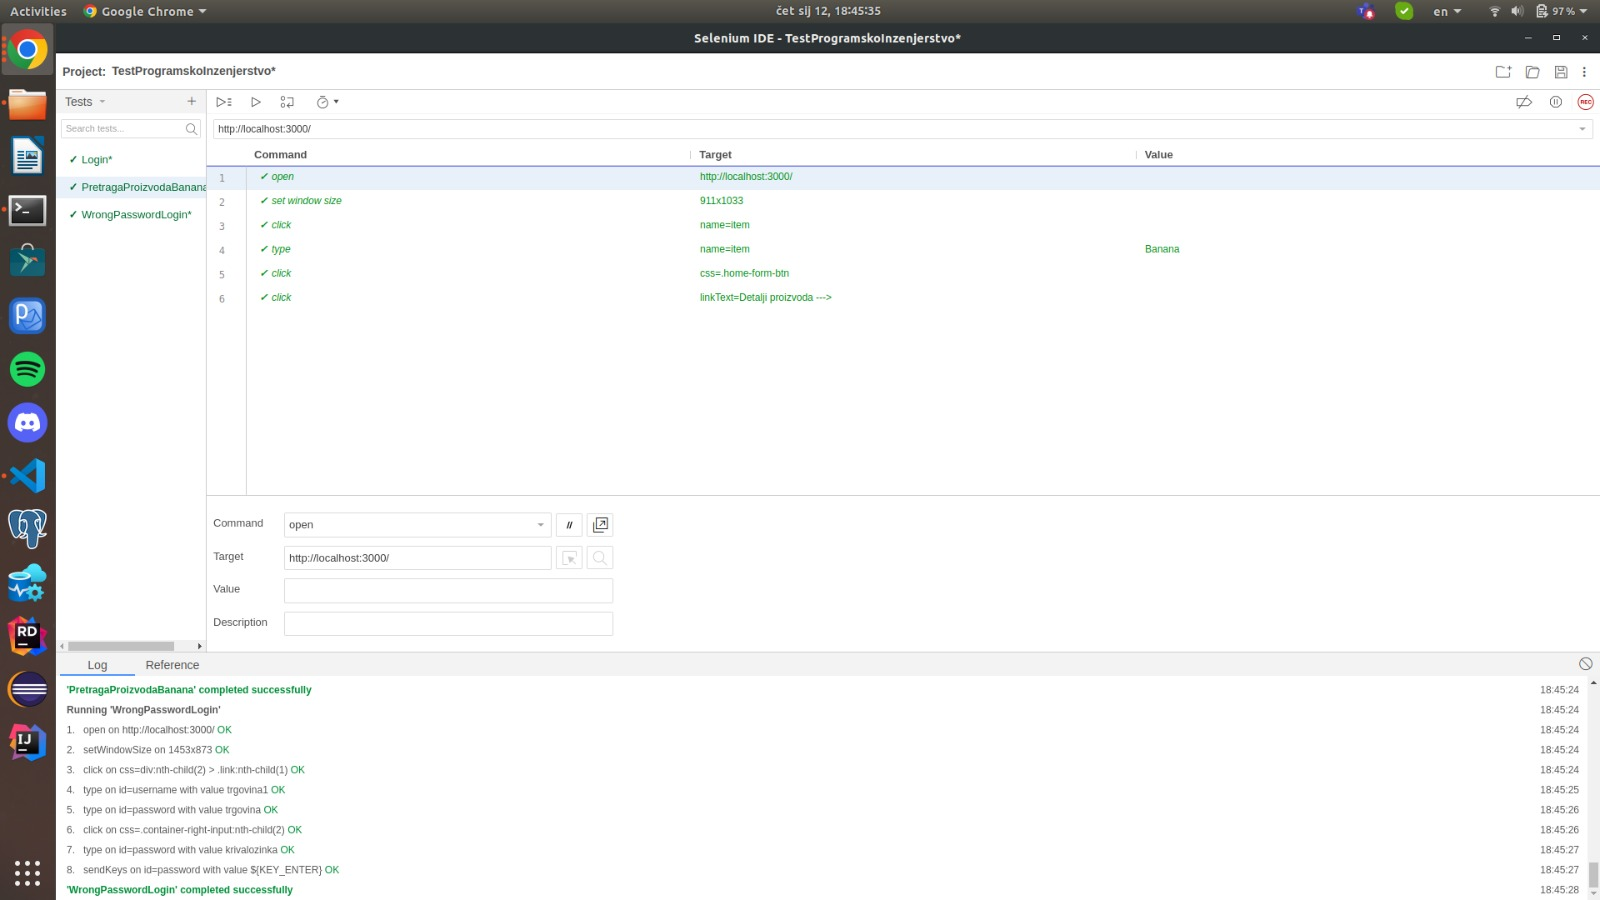
\includegraphics[width=\textwidth]{slike/sel3b.jpeg} %veličina u odnosu na širinu linije
			\caption{Selenium test 3, popis koraka}
			\label{fig:sel3b} %label mora biti drugaciji za svaku sliku
			\end{figure}
			
			Četvrti \textit{Selenium} test provodio se za funkcionalnosti pretrage trgovina. Konkretno testirali smo pretraživanje trgovina koje prodaju banane.
			
			\begin{figure}[H]
			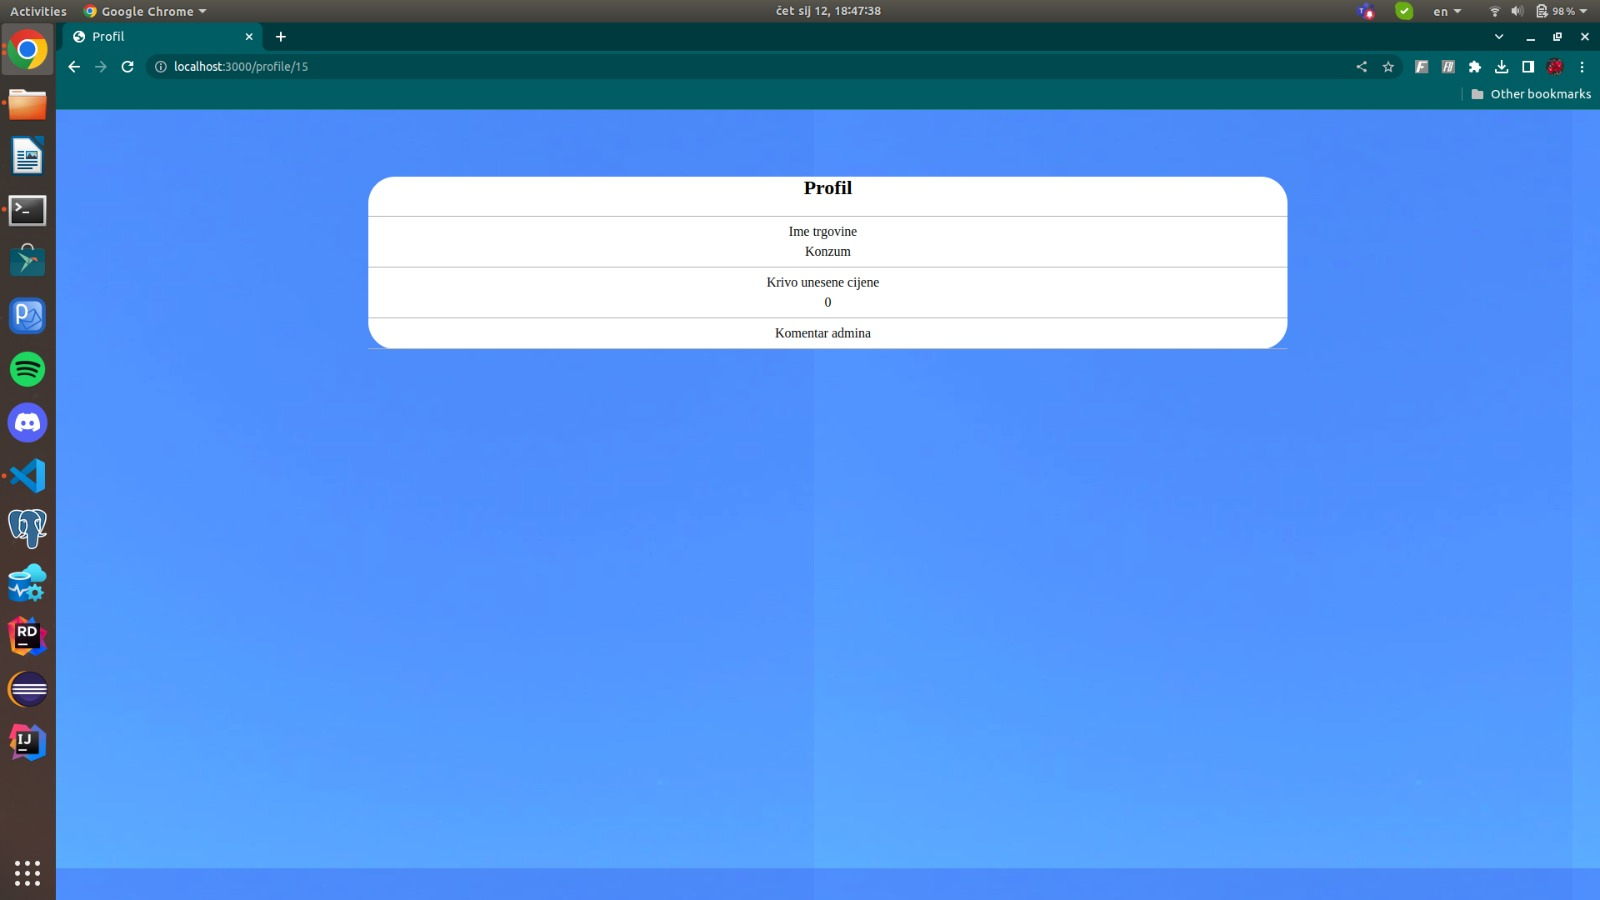
\includegraphics[width=\textwidth]{slike/sel4a.jpeg} %veličina u odnosu na širinu linije
			\caption{Selenium test 4, izgled sučelja}
			\label{fig:sel4a} %label mora biti drugaciji za svaku sliku
			Također, i ovaj test je uspješan.
			\end{figure}
			\begin{figure}[H]
			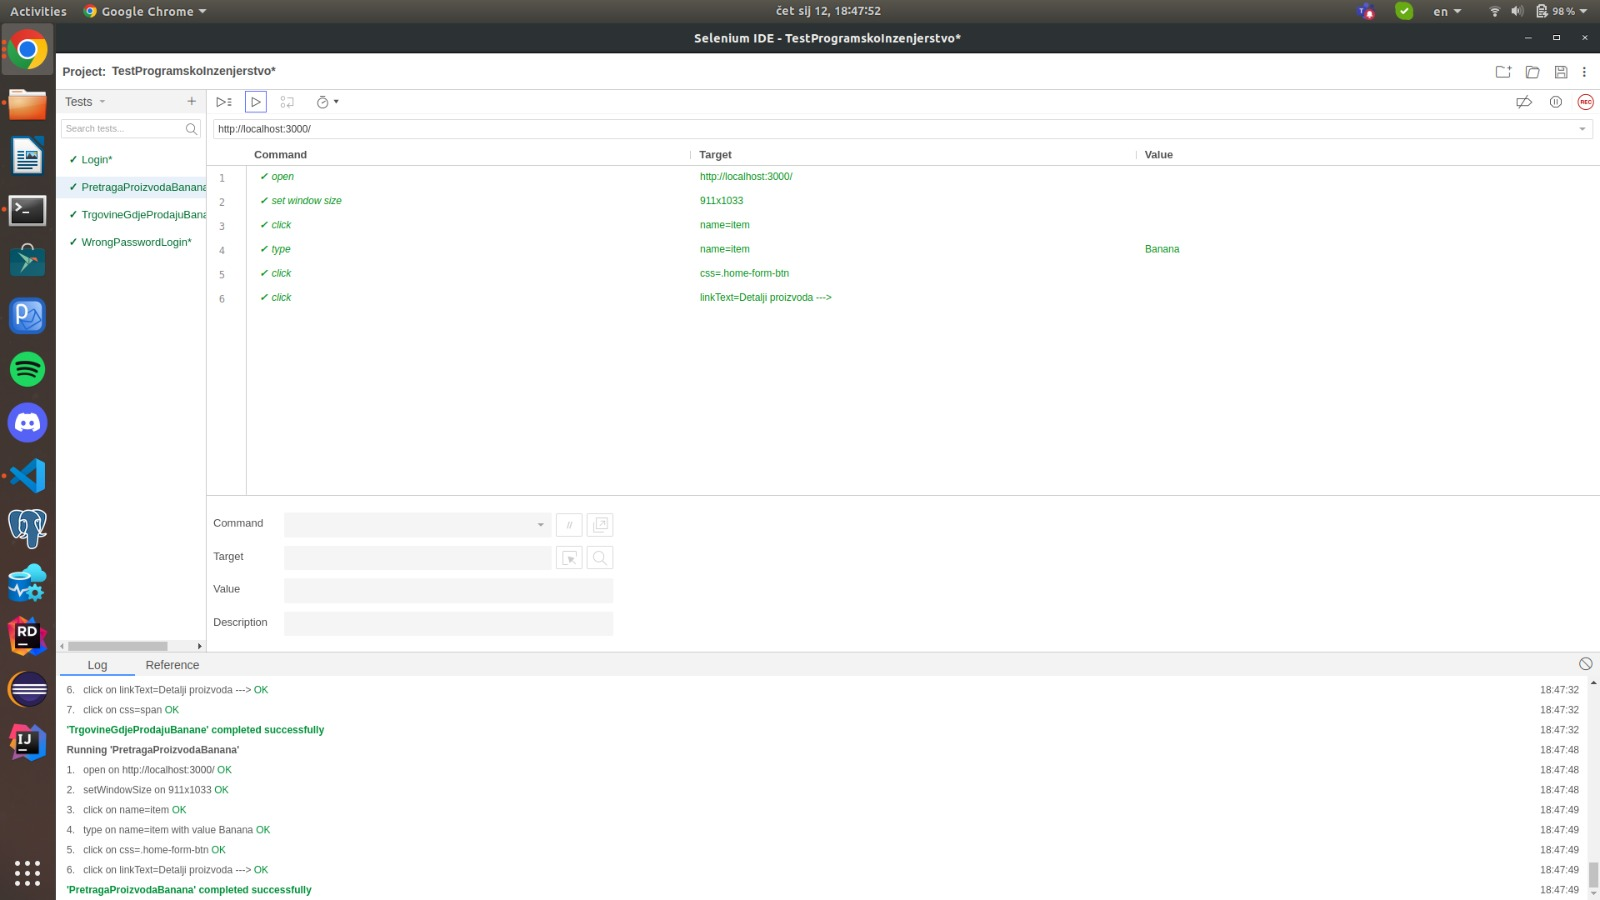
\includegraphics[width=\textwidth]{slike/sel4b.jpeg} %veličina u odnosu na širinu linije
			\caption{Selenium test 4, popis koraka}
			\label{fig:sel4b} %label mora biti drugaciji za svaku sliku
			\end{figure}
			
			\eject 
		
		
		\section{Dijagram razmještaja}
			
			%\textbf{\textit{dio 2. revizije}}
			
			 %\textit{Potrebno je umetnuti \textbf{specifikacijski} dijagram razmještaja i opisati ga. Moguće je umjesto specifikacijskog dijagrama razmještaja umetnuti dijagram razmještaja instanci, pod uvjetom da taj dijagram bolje opisuje neki važniji dio sustava.}
			 Na oblaku (eng. \textit{cloud}) pokrenuti su poslužitelji (eng. \textit{servers}) web-stranice i baze podataka koji međusobno komuniciraju, odnosno web-aplikacija sprema podatke u bazu. Korisnik sa svog računala preko web-preglednika pomoću HTTP protokola pristupa aplikaciji.
			 
			 \begin{figure}[H]
			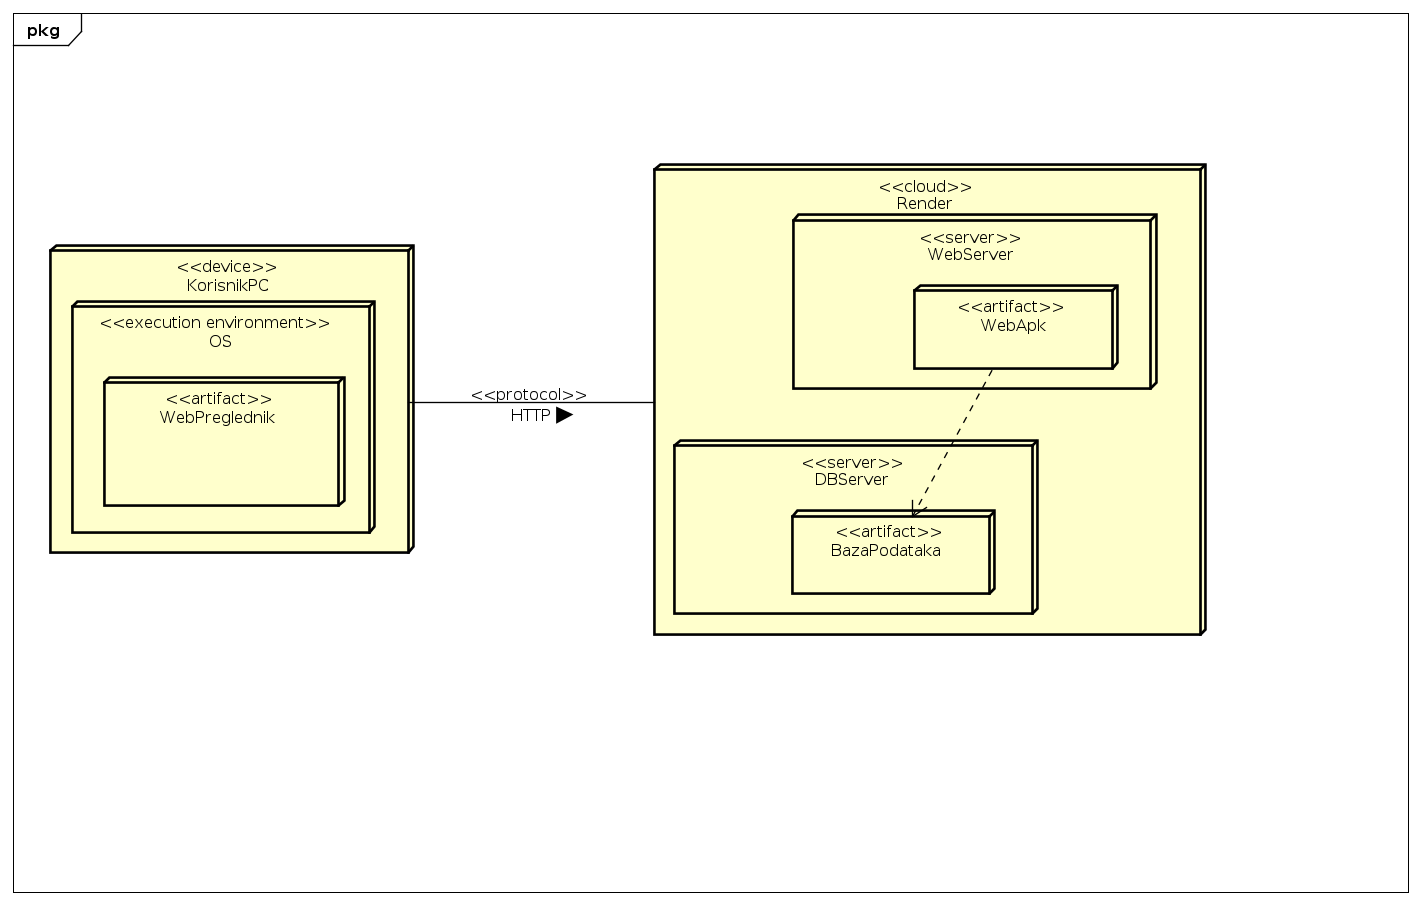
\includegraphics[width=\textwidth]{slike/dijagramRazmjestaja.png} %veličina u odnosu na širinu linije
			\caption{dijagram razmještaja}
			\label{fig:dijagramRazmjestaja} %label mora biti drugaciji za svaku sliku
			\end{figure}
			
			\eject 
		
		\section{Upute za puštanje u pogon}
		
			%\textbf{\textit{dio 2. revizije}}\\
		
			 %\textit{U ovom poglavlju potrebno je dati upute za puštanje u pogon (engl. deployment) ostvarene aplikacije. Na primjer, za web aplikacije, opisati postupak kojim se od izvornog kôda dolazi do potpuno postavljene baze podataka i poslužitelja koji odgovara na upite korisnika. Za mobilnu aplikaciju, postupak kojim se aplikacija izgradi, te postavi na neku od trgovina. Za stolnu (engl. desktop) aplikaciju, postupak kojim se aplikacija instalira na računalo. Ukoliko mobilne i stolne aplikacije komuniciraju s poslužiteljem i/ili bazom podataka, opisati i postupak njihovog postavljanja. Pri izradi uputa preporučuje se \textbf{naglasiti korake instalacije uporabom natuknica} te koristiti što je više moguće \textbf{slike ekrana} (engl. screenshots) kako bi upute bile jasne i jednostavne za slijediti.}
			
			
			 %\textit{Dovršenu aplikaciju potrebno je pokrenuti na javno dostupnom poslužitelju. Studentima se preporuča korištenje neke od sljedećih besplatnih usluga: \href{https://aws.amazon.com/}{Amazon AWS}, \href{https://azure.microsoft.com/en-us/}{Microsoft Azure} ili \href{https://www.heroku.com/}{Heroku}. Mobilne aplikacije trebaju biti objavljene na F-Droid, Google Play ili Amazon App trgovini.}
			 
			 \textbf{Prijava na sustav Render}\\
			 
			 
			 Web-aplikaciju je potrebno ugostiti (eng. \textit{to host}) na server kako bi bila dostupna svima. Kao servis za to odabran je \textbf{Render}. Za početak, potrebno je napraviti profil na stranici \underline{Render}\footnote{\url{https://render.com/}}.
			 \begin{figure}[H]
			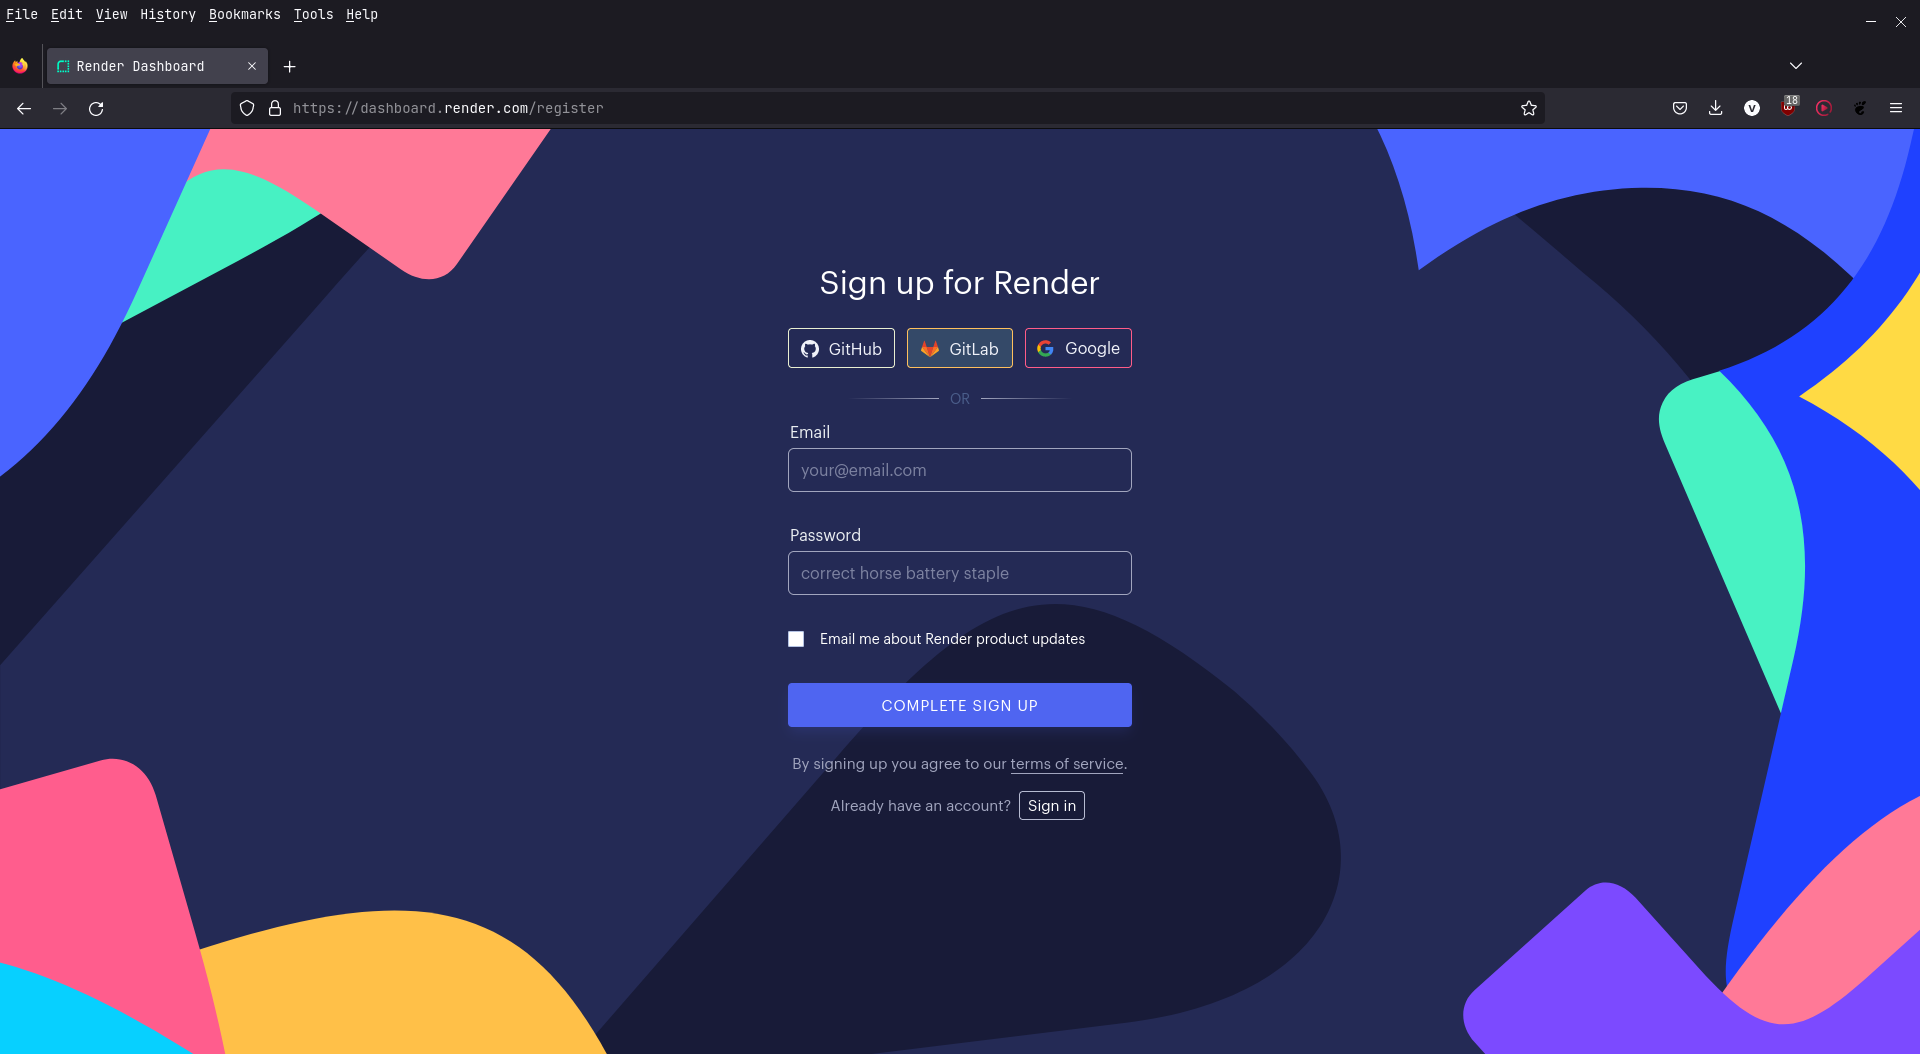
\includegraphics[width=\textwidth]{slike/signup.png} %veličina u odnosu na širinu linije
			\caption{forma za registraciju na Render}
			\label{fig:signup} %label mora biti drugaciji za svaku sliku
			\end{figure}
			 
			 
			 \textbf{Konfiguracija baze podataka}\\
			 
			 
			Kada smo se registrirali, potrebno je konfigurirati bazu podataka. Na \textit{Dashboardu} odabrati opcije \textbf{New} pa \textbf{New PostgreSQL}. Formu ispunimo na proizvoljan način, verziju ostavimo na 15. U ovom koraku bitno je zapisati si nazive u poljima \textbf{Database} i \textbf{User}. 
			\begin{figure}[H]
			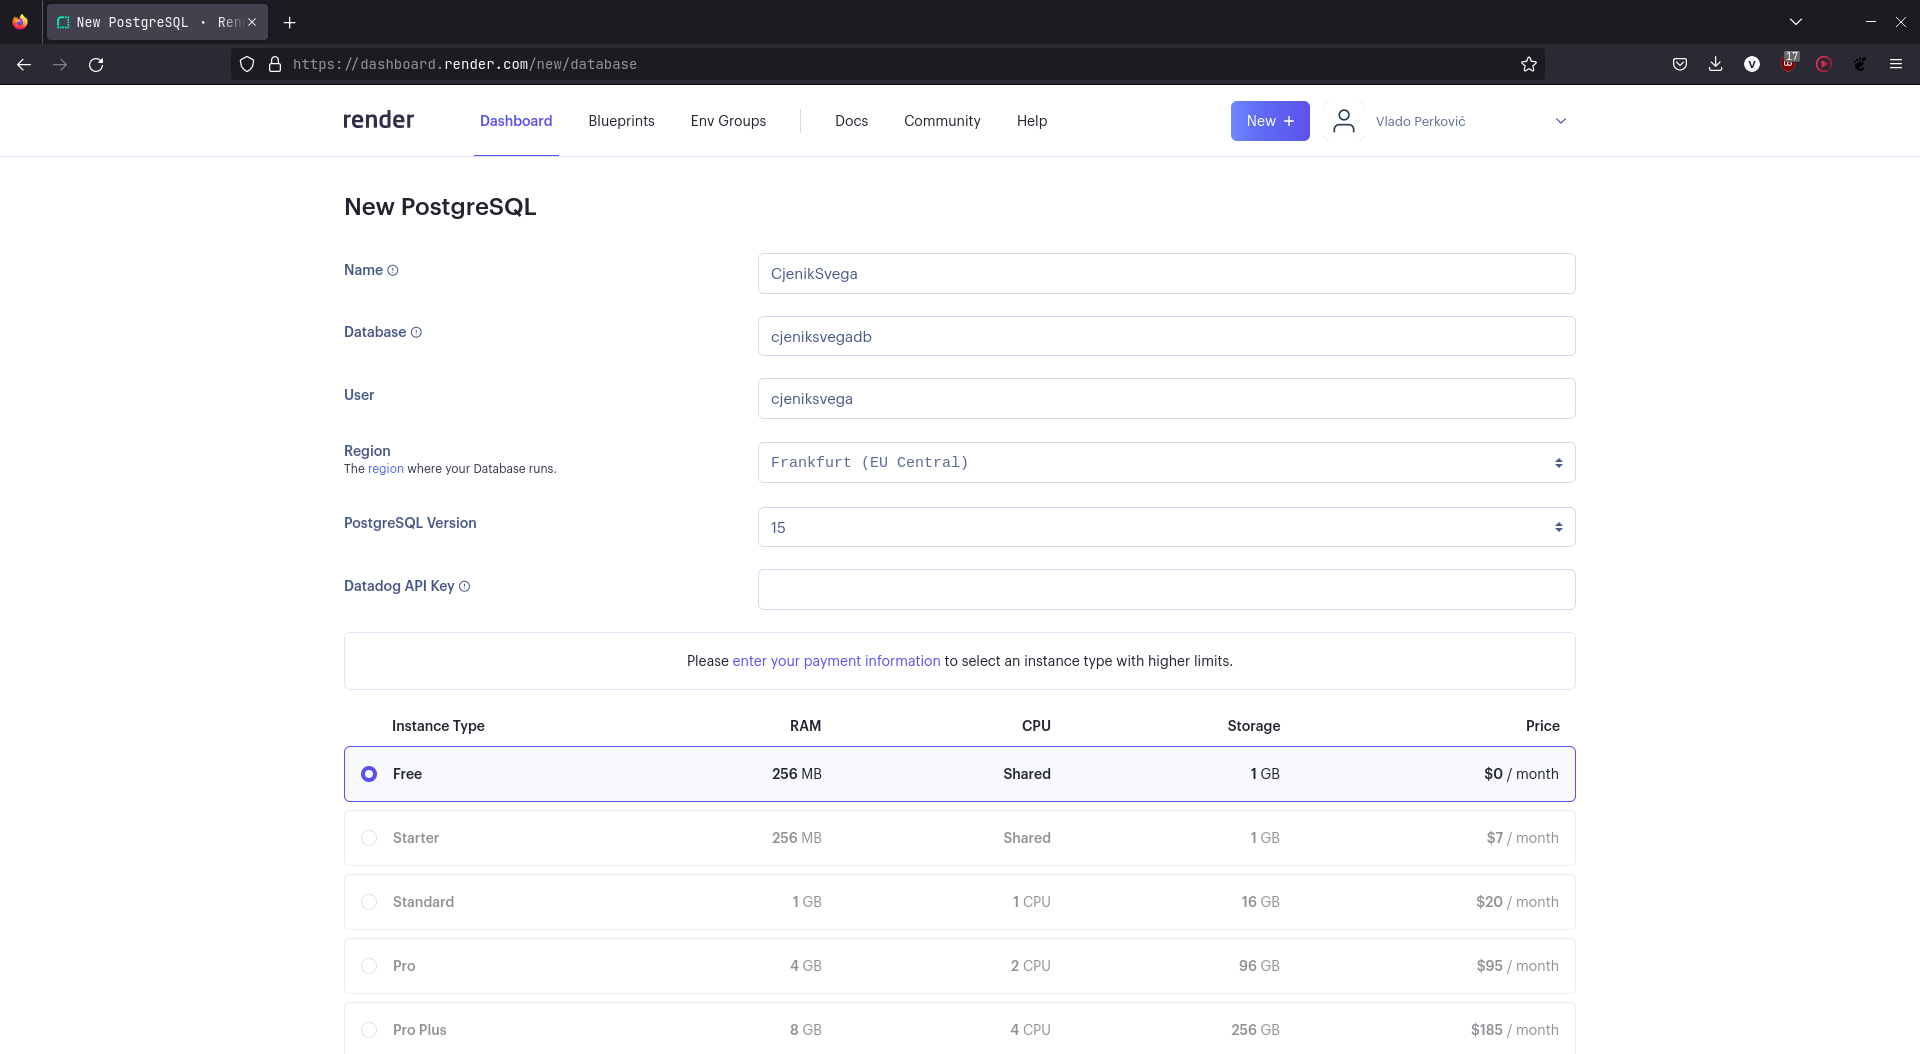
\includegraphics[width=\textwidth]{slike/konfigdb.png} %veličina u odnosu na širinu linije
			\caption{forma za konfiguraciju baze podataka}
			\label{fig:konfigdb} %label mora biti drugaciji za svaku sliku
			\end{figure}
			Nastavimo dalje pritiskom na \textbf{Create database}.
			Pričekamo da se baza napravi te pronađemo ju na \textit{Dashboardu} ukoliko se nije automatski otvorilo. Zapišemo si sa strane vrijednosti iz polja \textbf{Hostname}, \textbf{Port} i \textbf{Password}.\\
			
			
			\textbf{Konfiguracija web-servisa}\\
			
			
			Nakon uspješne konfiguracije baze podataka, potrebno je konfigurirati web-servis. Klikom na \textbf{New} pa \textbf{Web Service} otvaramo novo sučelje. Ako je repozitorij javan, pri dnu stranice potrebno je upisati poveznicu na Gitlab repozitorij i pritisnuti \textbf{Continue}. U slučaju da je repozitorij privatan, potrebno je spojiti git profil koji ima pristup projektu, nakon čega će biti ponuđen repozitorij CjenikSvega te potrebno je pritisnuti na \textbf{Connect}.
			\begin{figure}[H]
			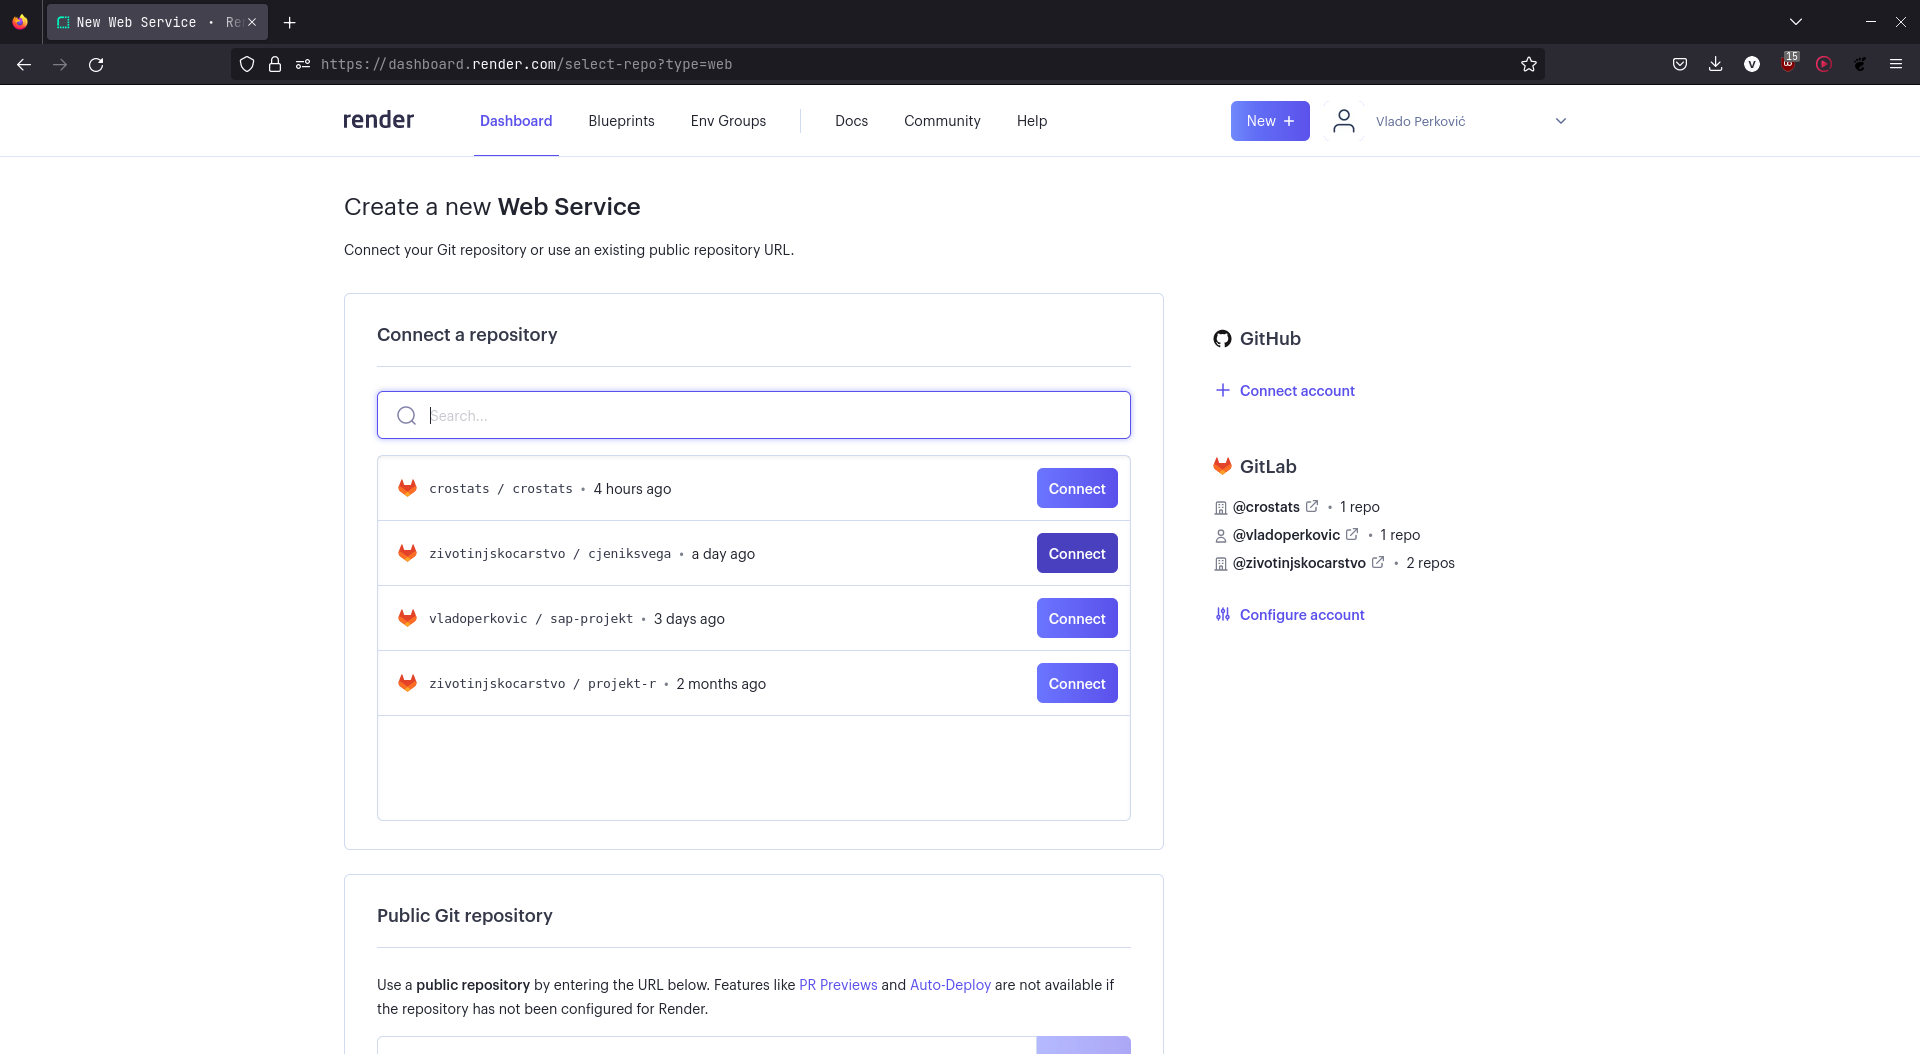
\includegraphics[width=\textwidth]{slike/connectweb.png} %veličina u odnosu na širinu linije
			\caption{spajanje na Gitlab repozitorij}
			\label{fig:gitlabConnect} %label mora biti drugaciji za svaku sliku
			\end{figure}
			
			U narednoj formi potrebno je navesti: 
			\begin{itemize}
		\item Name: CjenikSvega (proizvoljno jedinstveno ime)
\item Region: Frankfurt (preferira se najbliža)
\item Branch: master
\item Root Directory: IzvorniKod
\item Environment: Node
\item Build Command: \$ npm install
\item Start Command: \$ node ./db/seedDatabase.js
		\end{itemize}
		\begin{figure}[H]
			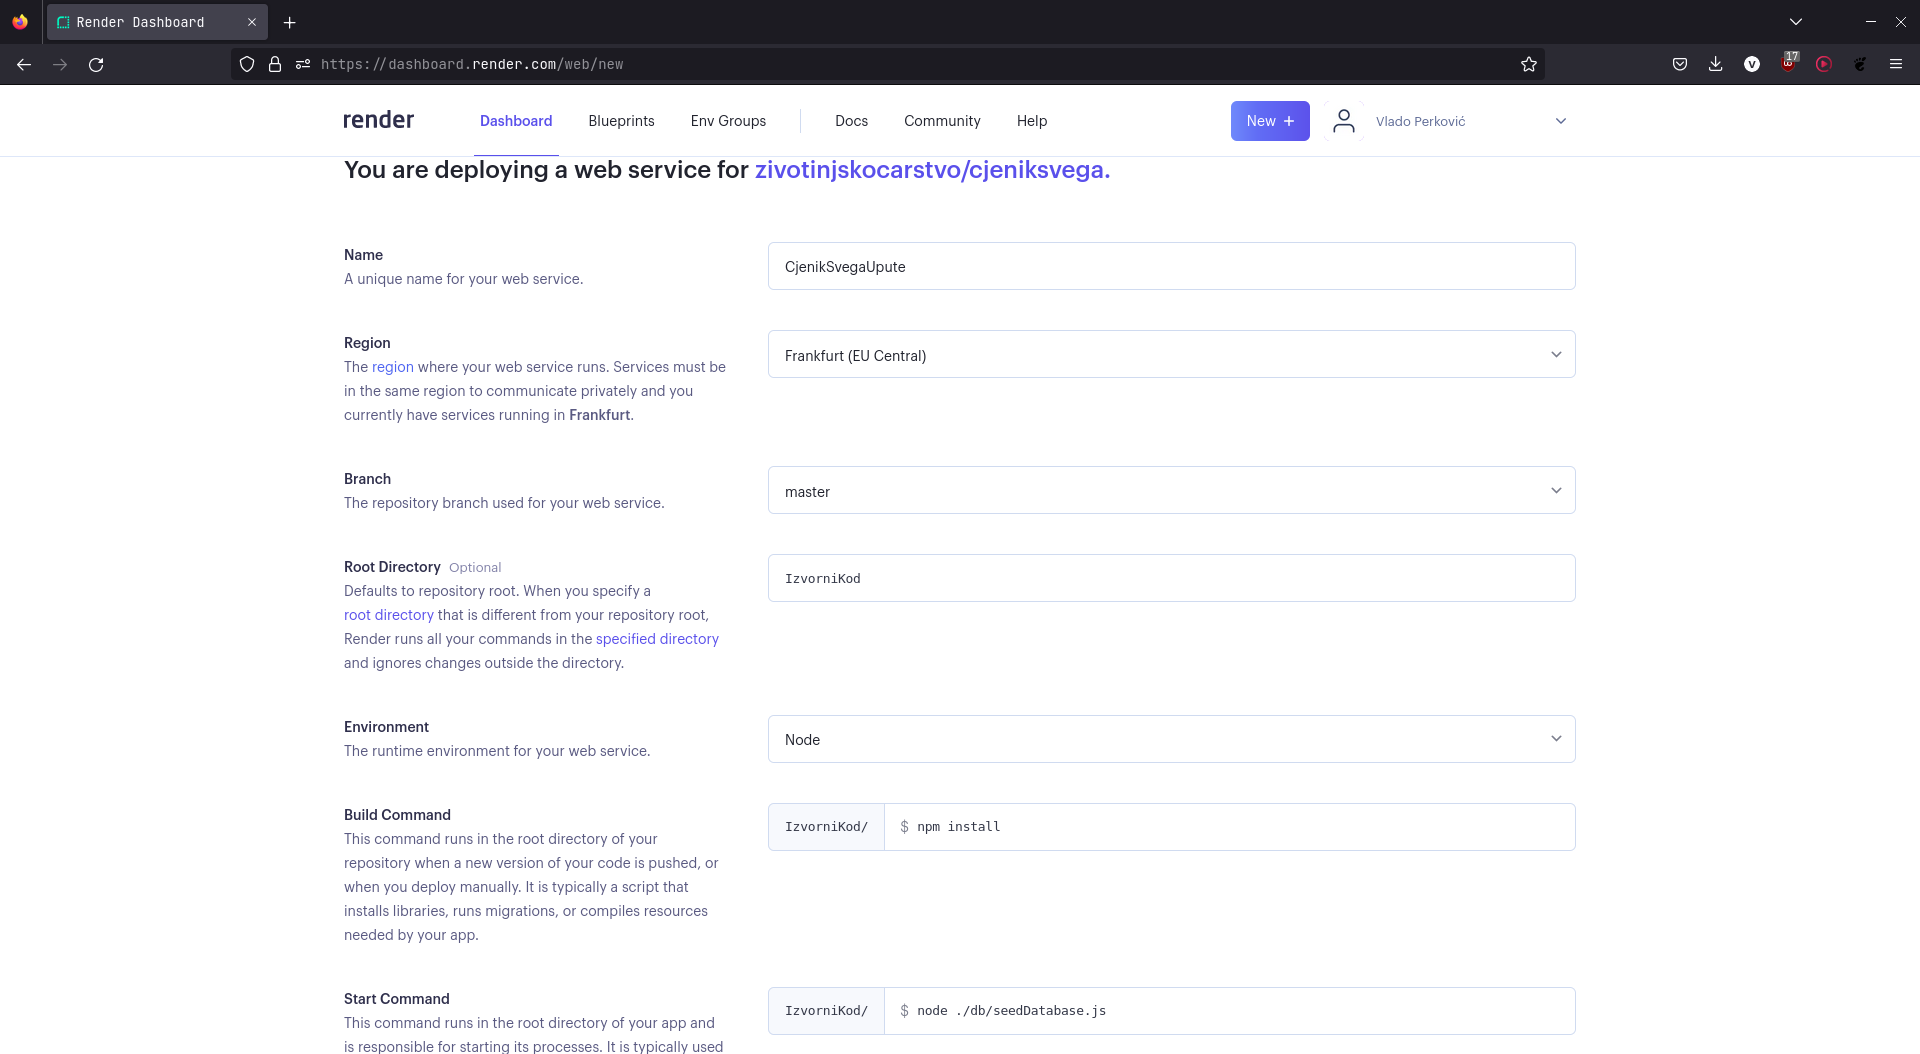
\includegraphics[width=\textwidth]{slike/konfigws.png} %veličina u odnosu na širinu linije
			\caption{ispunjavanje forme za web-servis}
			\label{fig:webservis} %label mora biti drugaciji za svaku sliku
			\end{figure}
			
			Potrebno je pritisnuti na \textbf{Advanced} i dodati environment varijable pritiskom na \textbf{Add Environment Variable}: dbHost, dbPort, dbName, dbUser i dbPassword s vrijednostima koje smo prije zapisali.
			\begin{figure}[H]
			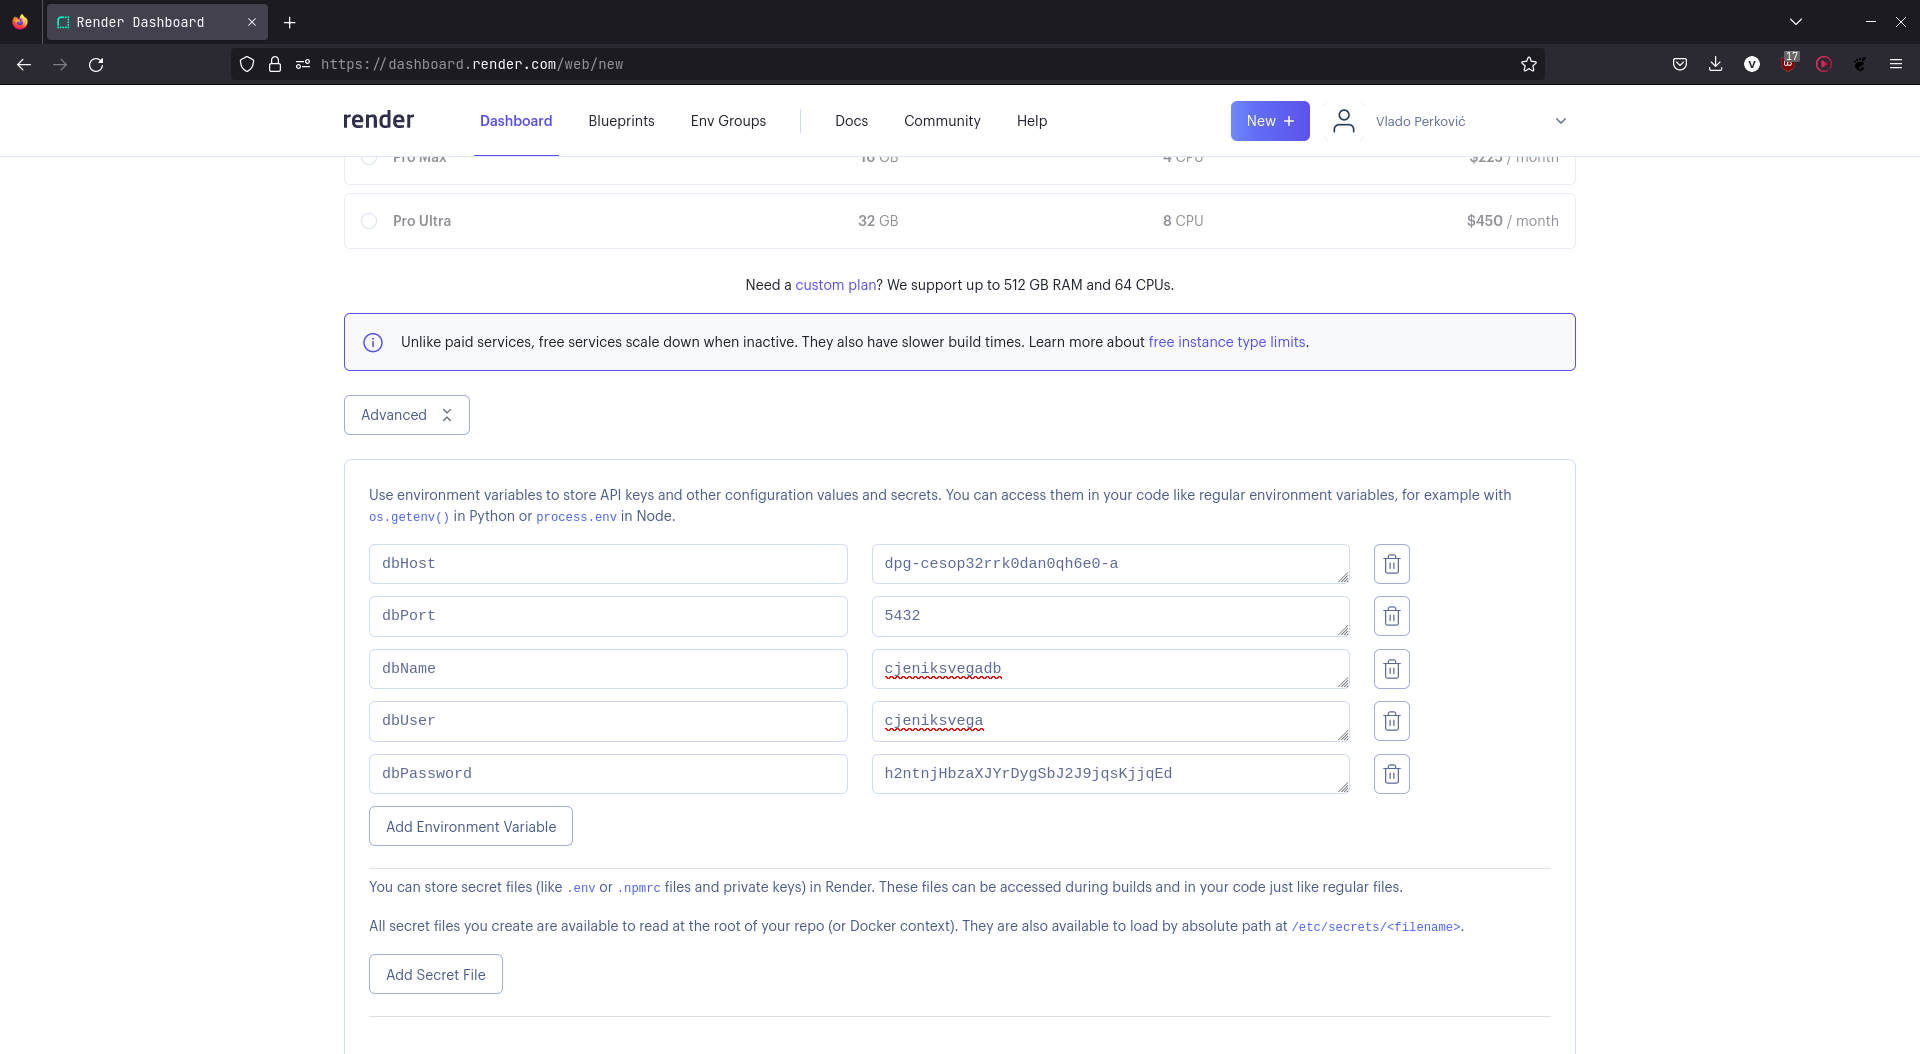
\includegraphics[width=\textwidth]{slike/envvar.png} %veličina u odnosu na širinu linije
			\caption{Podešavanje \textit{environment} varijabli}
			\label{fig:envvar} %label mora biti drugaciji za svaku sliku
			\end{figure}
			Na kraju pritisnemo \textbf{Create Web Service}.\\
			
			
			\textbf{Puštanje u pogon}\\
			
			
			Sada je potrebno pričekati da se baza kreira. Ako se nije automatski otvorio terminal, potrebno je pritisnuti na \textbf{Event} pa \textbf{Deploy} kako bismo mogli pratiti promjene. Kada uđe u \textit{loop} znamo da je baza kreirana.
			
			\begin{figure}[H]
			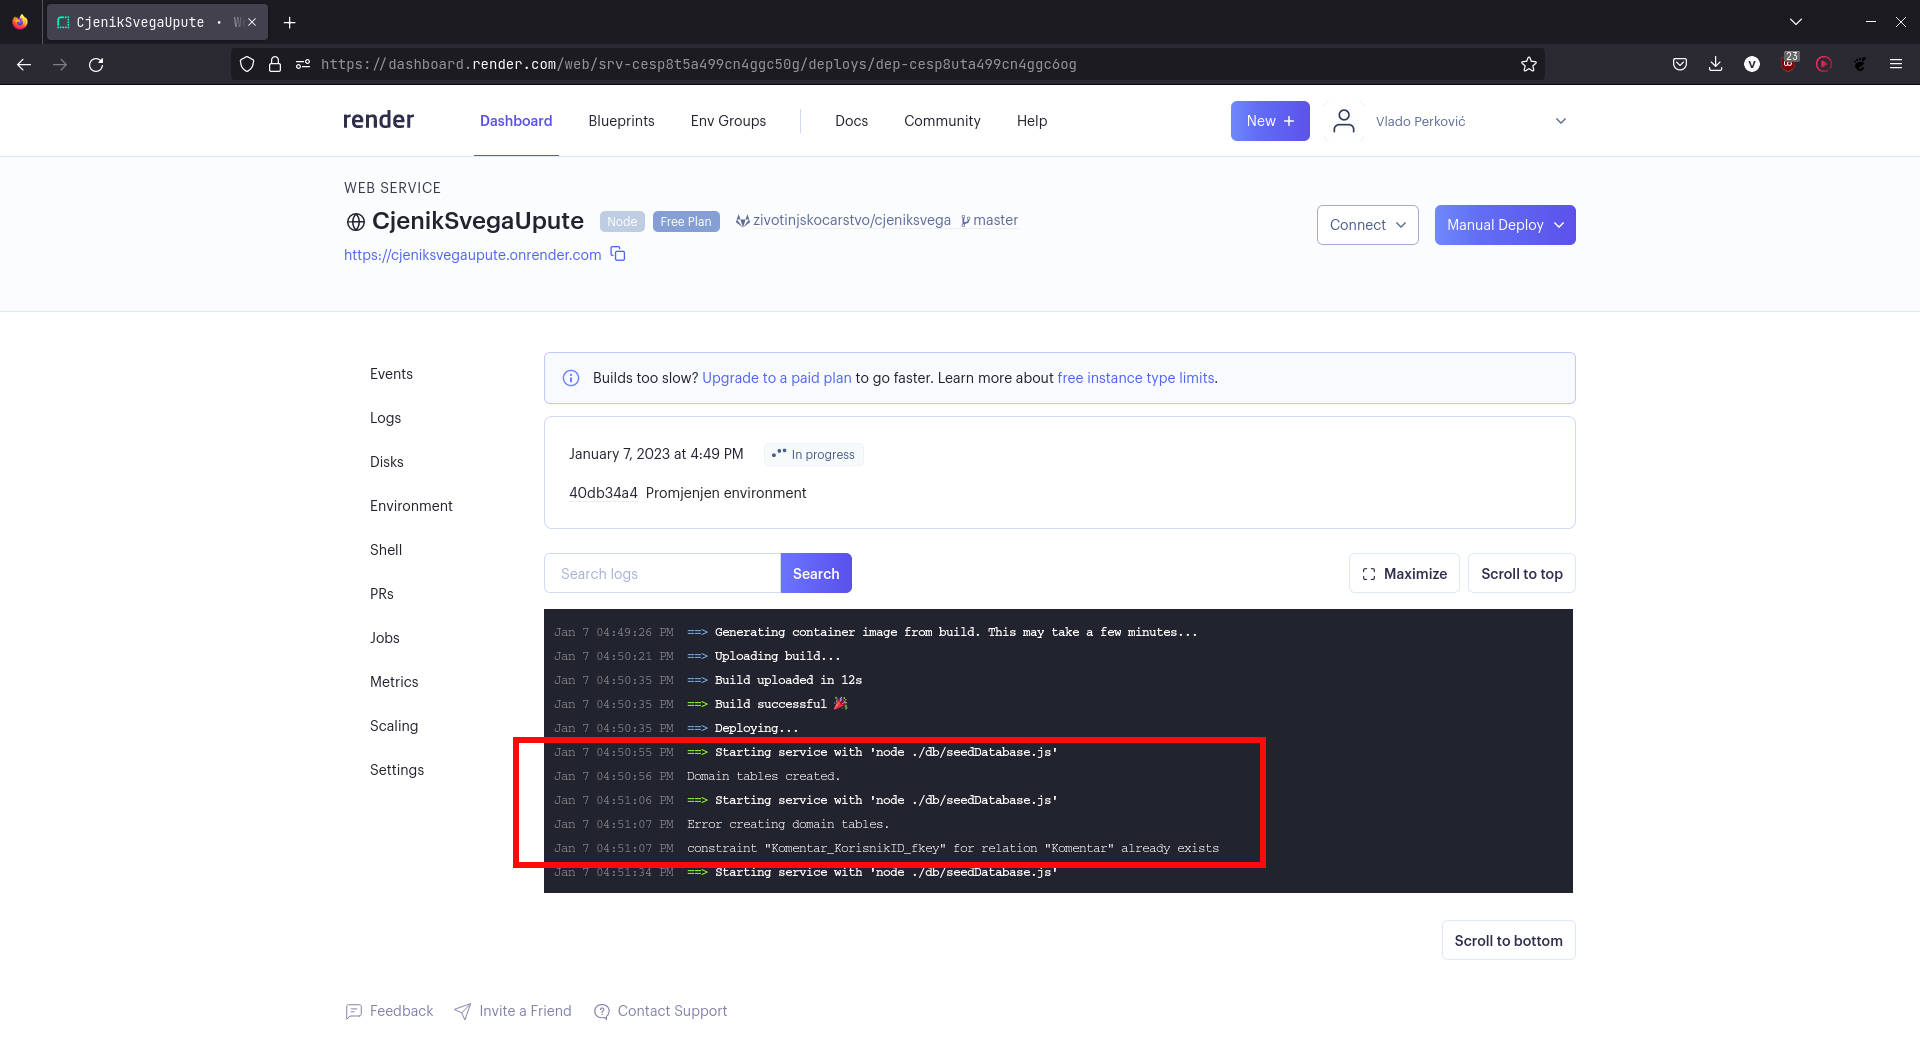
\includegraphics[width=\textwidth]{slike/seeddb.png} %veličina u odnosu na širinu linije
			\caption{Kreiranje baze}
			\label{fig:seeddb} %label mora biti drugaciji za svaku sliku
			\end{figure}
			
			Zatim je potrebno pritisnuti na \textbf{Settings} i promijeniti (eng. \textit{edit}) \textbf{Start Command} u \textbf{\$ npm server.js}.
			Kada promijenimo potrebno je pohraniti promjene (eng. \textit{Save Changes}) i vratiti se na \textbf{Event}.
			\begin{figure}[H]
			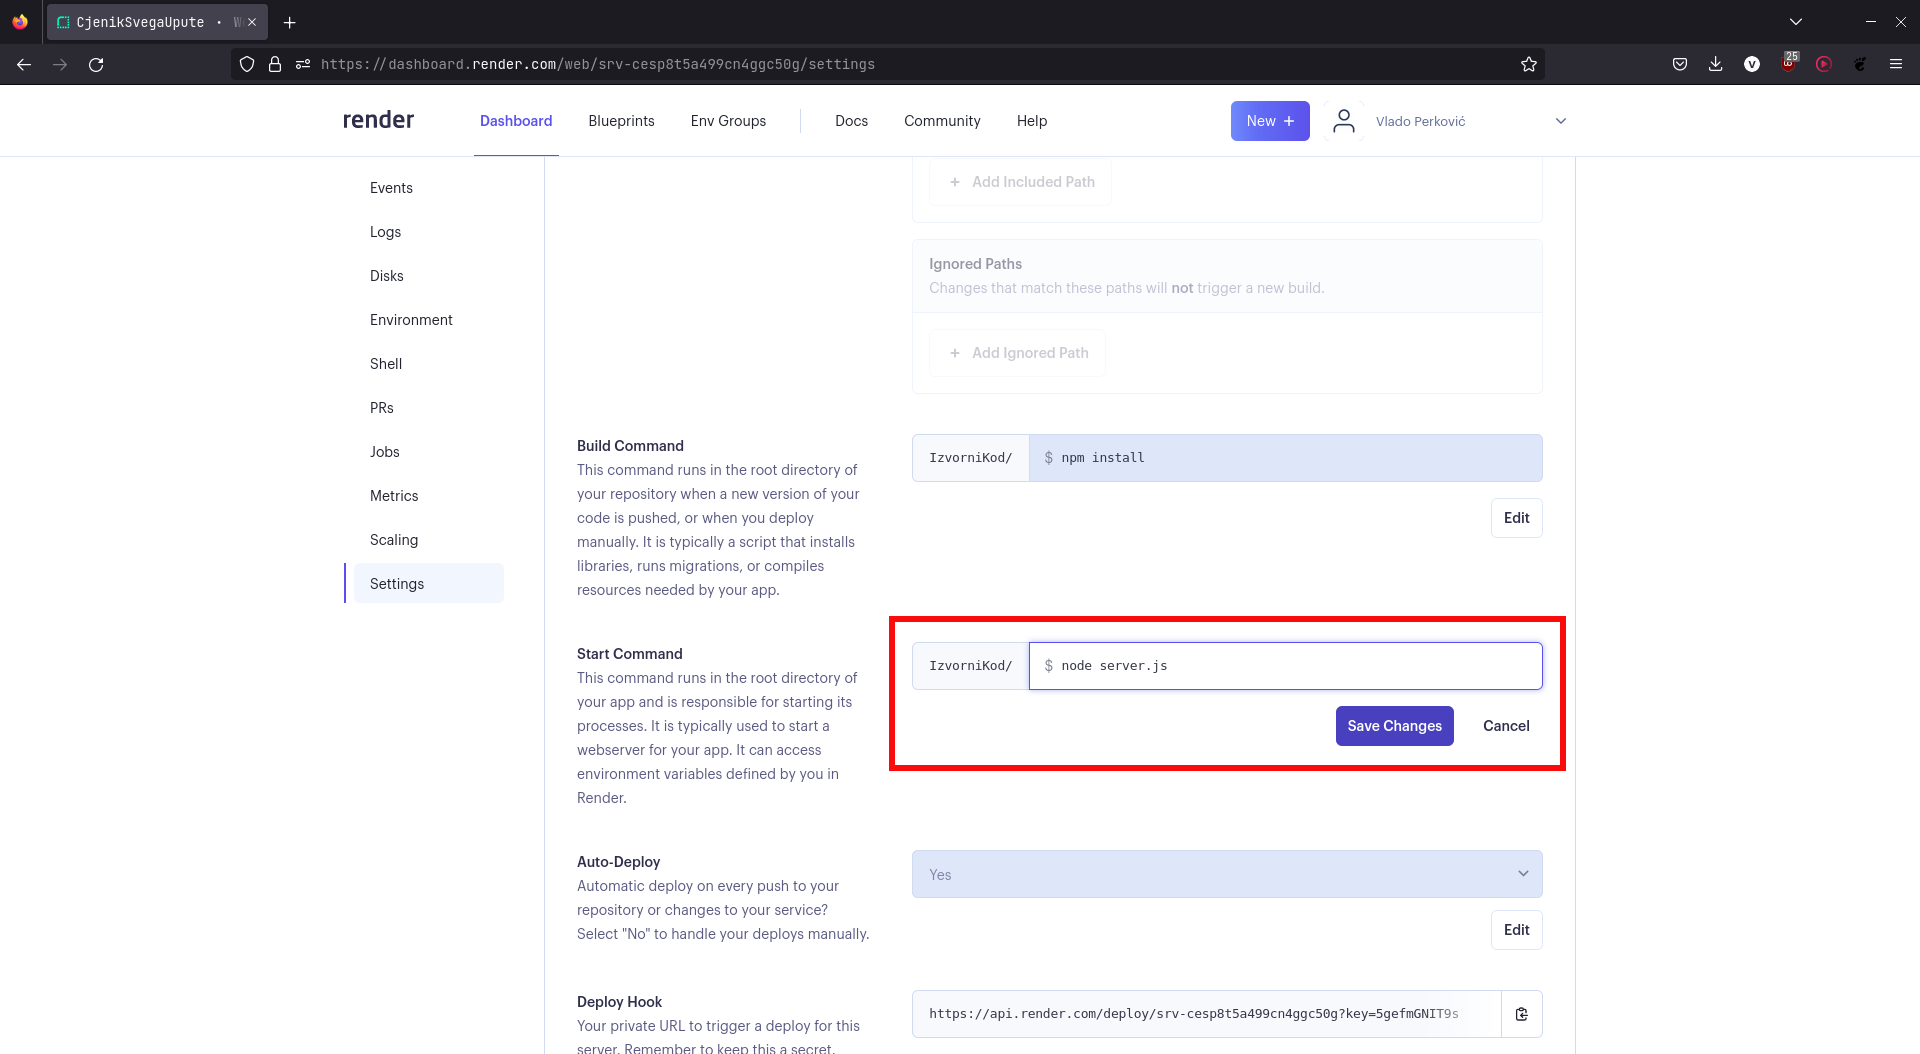
\includegraphics[width=\textwidth]{slike/serverjs.png} %veličina u odnosu na širinu linije
			\caption{Promjena \textit{Start Command}}
			\label{fig:serverjs} %label mora biti drugaciji za svaku sliku
			\end{figure}
			 Nakon nekoliko minuta web-aplikacija bi trebala biti dostupna na linku u gornjem lijevom kutu.
			 \begin{figure}[H]
			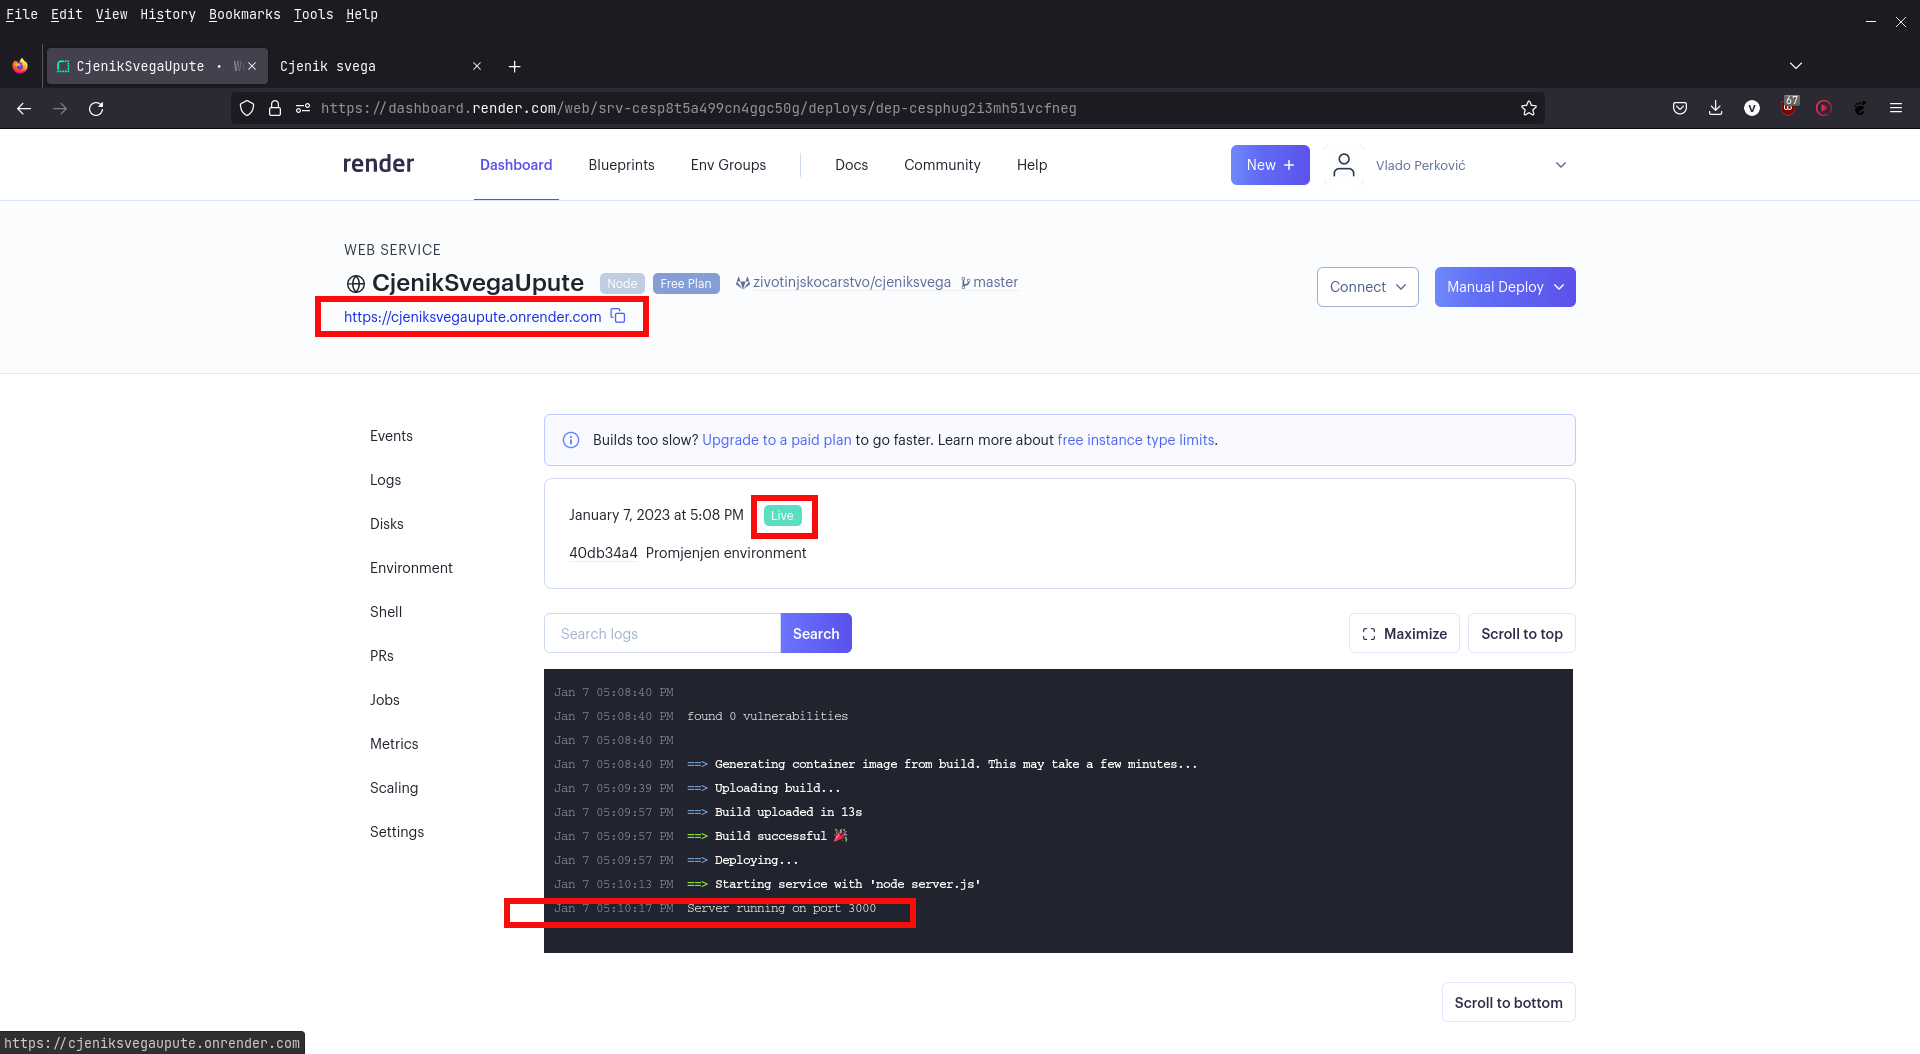
\includegraphics[width=\textwidth]{slike/deploy.png} %veličina u odnosu na širinu linije
			\caption{Uspješno puštanje u pogon}
			\label{fig:seeddb} %label mora biti drugaciji za svaku sliku
			\end{figure}
			
			
			\eject 